\documentclass[conference]{IEEEtran}
\IEEEoverridecommandlockouts
%Template version as of 6/27/2024

\usepackage{booktabs}
\usepackage{array}
\usepackage{tabularx}
\usepackage{listings}
\usepackage{xcolor}
\usepackage{placeins}
\usepackage{graphicx}
\usepackage{cite}
\usepackage{amsmath,amssymb,amsfonts}
\usepackage{algorithmic}
\usepackage{float}
\usepackage{textcomp}
\usepackage{url}
\usepackage{enumitem}

\lstset{
  basicstyle=\ttfamily\footnotesize,
  breaklines=true,
  breakatwhitespace=true,
  columns=fullflexible,
  frame=single,
  keepspaces=true
}

\def\BibTeX{{\rm B\kern-.05em{\sc i\kern-.025em b}\kern-.08em
    T\kern-.1667em\lower.7ex\hbox{E}\kern-.125emX}}
\begin{document}

\title{Internalizing MCP Tool Knowledge in Small LLMs via QLoRA Fine-Tuning}
\author{
\IEEEauthorblockN{1\textsuperscript{st} Tanmay Agarwal}
\IEEEauthorblockA{\textit{Columbia Engineering} \\
\textit{Columbia University}\\
NY, USA \\
ta2830@columbia.edu}
\and
\IEEEauthorblockN{2\textsuperscript{nd} Yuval Shemla}
\IEEEauthorblockA{\textit{Columbia School of General Studies} \\
\textit{Columbia University}\\
NY, USA \\
ys3571@columbia.edu}
\and
\IEEEauthorblockN{3\textsuperscript{rd} Ayal Yakobe}
\IEEEauthorblockA{\textit{Columbia Engineering} \\
\textit{Columbia University}\\
NY, USA \\
amy2127@columbia.edu}
}
\maketitle

%===========================================================================
\section{Introduction}
%===========================================================================

\subsection{Background}

Large language models (LLMs) are increasingly deployed as the backbone of modern agentic systems, where they orchestrate multi-step workflows involving tool use, reasoning, and interaction across multiple subtasks. In many current implementations---particularly within frameworks such as the Model Context Protocol (MCP) \cite{b1}---an LLM is tasked with both planning and execution. This typically requires the model to process extensive prompts that include full tool schemas and descriptions for every query. While effective, this approach is computationally inefficient and often relies on large frontier models, even when the task itself is fundamentally structured.

\subsection{Problem Statement}

This paradigm introduces two key inefficiencies. First, smaller models, such as those in the 2B--5B parameter range, often struggle to perform reliable tool planning without extensive prompting, forcing practitioners to rely on significantly larger and more expensive models. Second, current tool-use LLM agents commonly require detailed tool schemas to be included in every prompt. This repeated tool-context prompting creates substantial token overhead, increasing latency and operational cost. As observed in benchmarks such as AssetOpsBench \cite{b2}, this overhead can reach thousands of tokens per query and scales linearly with the number of tools. In our end-to-end execution setting, tool descriptions account for 82.6\% of the input tokens, making schema repetition the dominant source of prompt inefficiency.

\subsection{Contributions}

In this work, we address this limitation by shifting tool-use knowledge from the prompt into the model weights. We propose a fine-tuning pipeline that teaches smaller open-source models to internalize tool schemas, argument patterns, and planning strategies, enabling them to generate structured execution plans without explicit tool descriptions in the prompt---a setting we refer to as \emph{description-free} inference. Our main contributions are:

\begin{enumerate}[leftmargin=*, topsep=2pt, itemsep=1pt]
\item We show that QLoRA fine-tuning on $\sim$1,700 examples enables $\sim$4B parameter models to produce correct MCP tool-use plans \emph{without tool descriptions in the prompt}, surpassing the informed baseline on both structural metrics and LLM-judge scores.
\item We compare two architectures---Gemma 4 E4B (4.5B) and Qwen3-4B (4.0B)---and find that Qwen3 achieves higher planning quality with 62\% less memory and 2.5$\times$ faster inference.
\item We quantify catastrophic forgetting after tool-use fine-tuning and show that smaller LoRA ranks reduce degradation with minimal quality loss.
\item We profile the full training and inference pipeline on A100, identifying the 8-bit matrix multiplication kernel as the dominant bottleneck (56.3\% of CUDA time).
\end{enumerate}


%===========================================================================
\section{Literature Review}
%===========================================================================

To address this problem, we build on prior work in industrial tool-use benchmarks, standardized tool interfaces, and parameter-efficient fine-tuning.

\subsection{IBM Asset Operations Benchmark}

Asset Operations Benchmark (AssetOpsBench) is a benchmark and framework introduced by IBM Research for evaluating AI agents in industrial asset operations and maintenance \cite{b2}. It tests whether a model can interpret domain-specific operations queries and select the appropriate tools, agents, arguments, and execution order needed to answer them. AssetOpsBench includes human-authored natural-language scenarios, simulated industrial telemetry, domain-specific agents such as IoT, FMSR, TSFM, and work-order agents, and multi-agent evaluation protocols. In our work, we use AssetOpsBench as the primary benchmark for training data generation and evaluation, focusing on the 152 human-generated queries defined in the MCP setting \cite{b1}.

\subsection{LoRA and QLoRA}

Low-Rank Adaptation (LoRA) \cite{b4} is a parameter-efficient fine-tuning method that freezes the pretrained model weights and injects small trainable rank-decomposition matrices into each layer. QLoRA \cite{b3} extends this approach by additionally quantizing the frozen weights to 4-bit or 8-bit precision, further reducing memory requirements while preserving much of the performance of full fine-tuning. In our experiments, we use QLoRA with 8-bit quantization to fine-tune models in the 4--5B parameter range on a single A100 GPU.

\subsection{Catastrophic Forgetting in LoRA}

Because LoRA freezes the original model weights and trains only small adapter modules, it generally reduces catastrophic forgetting compared with full fine-tuning \cite{b7}. However, forgetting can still occur because the learned adapters modify the model's effective behavior at inference time, potentially biasing the model toward the fine-tuning task and degrading its general capabilities. This is particularly relevant for tool-use fine-tuning, where the training distribution (structured plans) differs substantially from the pretraining distribution (general text).

\subsection{Tool-Use LLM Literature}

There is substantial prior work on tool-use LLMs, in which language models are trained or prompted to decide when to use external tools, which tools to select, and what arguments to provide. This direction has been explored extensively in API-use settings, including Toolformer \cite{b8}, Gorilla \cite{b9}, and ToolLLM \cite{b10}. These approaches typically keep tool descriptions in the prompt or retrieve API documentation at inference time. Our work differs in that we train the model to internalize the tool catalog entirely, eliminating the need for any tool descriptions at inference time---a stricter form of tool knowledge than prior work requires. This trades generalization to unseen tools, which prompt-based approaches support by simply adding new descriptions, for inference efficiency on a fixed tool catalog.

\subsection{Knowledge Distillation and Prompt Compression}

Prompt compression methods such as LLMLingua \cite{b11} remove less important content from long prompts, while knowledge distillation approaches \cite{b12} train a smaller student model to reproduce the outputs or reasoning traces of a larger teacher model. Our approach can be viewed as an extreme form of prompt compression in which the entire tool-schema section is removed and its content is internalized into model weights via supervised fine-tuning. Unlike standard distillation, we do not require teacher model inference at test time.


%===========================================================================
\section{Methodology}
%===========================================================================

\subsection{Benchmark and Data}

We use AssetOpsBench \cite{b2} as the primary benchmark for both data construction and evaluation. The benchmark contains 152 natural-language scenarios, each requiring the model to select appropriate domain tools, generate valid arguments, and order tool calls into a structured execution plan. Each plan consists of sequenced steps in a structured format specifying a task description, the assigned agent, the tool to call, JSON arguments, and inter-step dependencies.

We construct training data using Gemini 2.5 Flash \cite{b5} as the teacher model, grounded in a tool catalog of five agents and 23 tools with full descriptions, argument schemas, and return types (Table~\ref{tab:compact-tool-inventory}). The resulting data comprises three types of supervised fine-tuning examples (see Appendix~A for composition). \emph{Tool and agent knowledge} examples teach the model which agents and tools exist, how they are associated, what arguments each tool requires, and how to distinguish between near-miss tools such as \texttt{get\_failure\_modes} and \texttt{get\_failure\_mode\_sensor\_mapping}. \emph{Question-to-plan} examples, based on the 152 AssetOpsBench scenarios together with generated paraphrases, teach the model to map a natural-language query to a structured plan; each plan is validated to follow the required \texttt{\#Task}/\texttt{\#Agent}/\texttt{\#Tool}/\texttt{\#Args} format. \emph{Execution-style} examples combine planning steps with execution traces and placeholder-resolution patterns such as \texttt{\{step\_N\}}.

At inference time, each query is embedded in a structured planning prompt (shown in full in Appendix~\ref{app:prompt-example}). The prompt contains: (1)~a system preamble describing the model's role as a planning assistant, (2)~the complete tool catalog listing all agents, their tools, argument signatures, and descriptions ($\sim$2,200 tokens), (3)~the structured output format specification (\texttt{\#Task}/\texttt{\#Agent}/\texttt{\#Tool}/\texttt{\#Args}/\texttt{\#Dependency}/\texttt{\#ExpectedOutput}), and (4)~the user question. In the description-free setting, section~(2) is removed entirely, reducing the prompt to $\sim$128 tokens.

For evaluation, we use a pattern-aware stratified 80/20 split over the 152 scenarios, where each scenario is assigned a pattern based on its type, tool set, and step count. This produces 122 training scenarios and 30 held-out test scenarios. The full training corpus contains approximately 1,833 examples. We define three training configurations: Config~A (Plan-only, $\sim$1,200 examples), Config~B (Tool-knowledge only, $\sim$500 examples), and Config~C (Tool+Plan, $\sim$1,741 examples). Config~C is used as the primary setting throughout unless otherwise noted.

\begin{table}[ht]
\centering
\caption{Tool inventory: 23 tools across five agent families}
\label{tab:compact-tool-inventory}
\begin{tabular}{lr}
\hline
Agent Family & Tools \\
\hline
IoTAgent & 4 \\
FMSRAgent & 2 \\
TSFMAgent & 6 \\
Utilities & 3 \\
WorkOrderAgent & 8 \\
\hline
\end{tabular}
\end{table}

\subsection{Models and Training}

We compare two open-source instruction-tuned models: Gemma 4 E4B-it \cite{b6} and Qwen3-4B \cite{b17}. Table~\ref{tab:model-summary} summarizes their architectural differences. Both share a hidden size of 2560 but differ in depth, attention mechanism, and vocabulary size.

\begin{table}[t]
\centering
\caption{Base models used for fine-tuning}
\label{tab:model-summary}
\footnotesize
\begin{tabular}{lcc}
\hline
 & \textbf{Gemma 4 E4B} & \textbf{Qwen3-4B} \\
\hline
Total params & $\sim$8B (with PLE) & 4.0B \\
Active params & 4.5B effective & 3.6B \\
Layers & 42 & 36 \\
Attention & Hybrid (36 slide + 6 global) & GQA (32Q / 8KV) \\
Hidden size & 2560 & 2560 \\
Vocab size & 262K & 152K \\
\hline
\end{tabular}
\end{table}

Both models are fine-tuned using QLoRA with 8-bit quantization, which keeps the base model weights fixed while training a small set of adapter parameters. We use the same Config~C dataset for both models (1,741 training, 92 evaluation examples) and train with identical hyperparameters: LoRA rank $r=32$, $\alpha=64$, dropout $0.05$, learning rate $2 \times 10^{-4}$ with cosine schedule, batch size $2$ with gradient accumulation of $4$, $2$ epochs, early stopping with patience $2$, and $436$ total training steps. All linear layers are targeted.

Although the two models use the same LoRA rank, the resulting trainable-parameter fraction differs due to model-size differences. For Gemma, rank $32$ corresponds to approximately $0.63\%$ trainable parameters, whereas for Qwen3 it corresponds to approximately $1.62\%$---about $2.6\times$ higher adaptation intensity. This difference directly affects forgetting, as discussed in Section~\ref{sec:forgetting}.


\subsection{Evaluation}

We evaluate plans using two complementary approaches. Structural metrics provide deterministic, reproducible scores but can penalize valid plans that deviate from the gold reference. LLM-based judging captures semantic quality and accepts valid alternative formulations, but may exhibit grading bias. Using both approaches and checking for agreement provides more robust evidence than either alone.

For structural evaluation, we report AT-F1, which extracts the set of (agent, tool) pairs from actionable steps (excluding steps where agent or tool is ``none'') in both the gold and candidate plans and computes set-based F1 (precision $=$ matched pairs / candidate pairs, recall $=$ matched pairs / gold pairs). We also report ArgKey-F1, which measures whether the model predicts the correct argument field names for matched tool calls. For semantic evaluation, we use Gemini 2.5 Flash as an LLM-as-judge \cite{b13} to rate each plan on six dimensions---correctness, agent routing, tool selection, argument quality, efficiency, and dependency correctness---on a 1--5 scale. The judge overall score is the mean of all six dimensions. Full judge prompts are in Appendix~E.

We evaluate models under three prompting conditions: \emph{informed}, where full tool descriptions are included in the prompt; \emph{description-free}, where the base model receives only the user query with no tool schemas; and \emph{fine-tuned description-free}, where the fine-tuned model generates plans without tool schemas at inference time.

We also evaluate catastrophic forgetting using 100 multiple-choice questions drawn from MMLU \cite{b14}, ARC-Challenge \cite{b15}, and HellaSwag \cite{b16}. Each model generates up to 512 tokens with chain-of-thought reasoning, and Gemini 2.5 Flash judges whether the final answer is correct. Details are in Appendix~F.

For profiling, we use the PyTorch Profiler, \texttt{torch.cuda} memory tracking, and Weights \& Biases. Full profiling details are in Appendix~D.


%===========================================================================
\section{Experimental Results}
%===========================================================================

\subsection{Main Result: Internalization Works}
\label{sec:main-result}

We first evaluate whether fine-tuning can internalize tool-use knowledge that would otherwise need to be supplied in the prompt. We define two baselines using the \emph{unfine-tuned} Gemma~4~E4B model. In the \emph{informed baseline}, the model receives a structured planning prompt containing a system preamble, the complete tool catalog with all agent names, tool signatures, argument types, and natural-language descriptions ($\sim$2,200 tokens of schema text), the output format specification, and the user query---totaling approximately 2,400 input tokens per query (see Appendix~\ref{app:prompt-example} for a concrete example). In the \emph{description-free baseline}, the same unfine-tuned model receives only the user query with no tool descriptions ($\sim$128 tokens). The description-free baseline achieves zero AT-F1, confirming that the base model cannot plan without explicit tool descriptions.

Fine-tuning changes this substantially. Figs.~\ref{fig:main-results} and~\ref{fig:judge-scores} show that both fine-tuned models perform well in the description-free setting and, crucially, \emph{outperform} the informed baseline on every metric.

\begin{figure}[t]
\centering
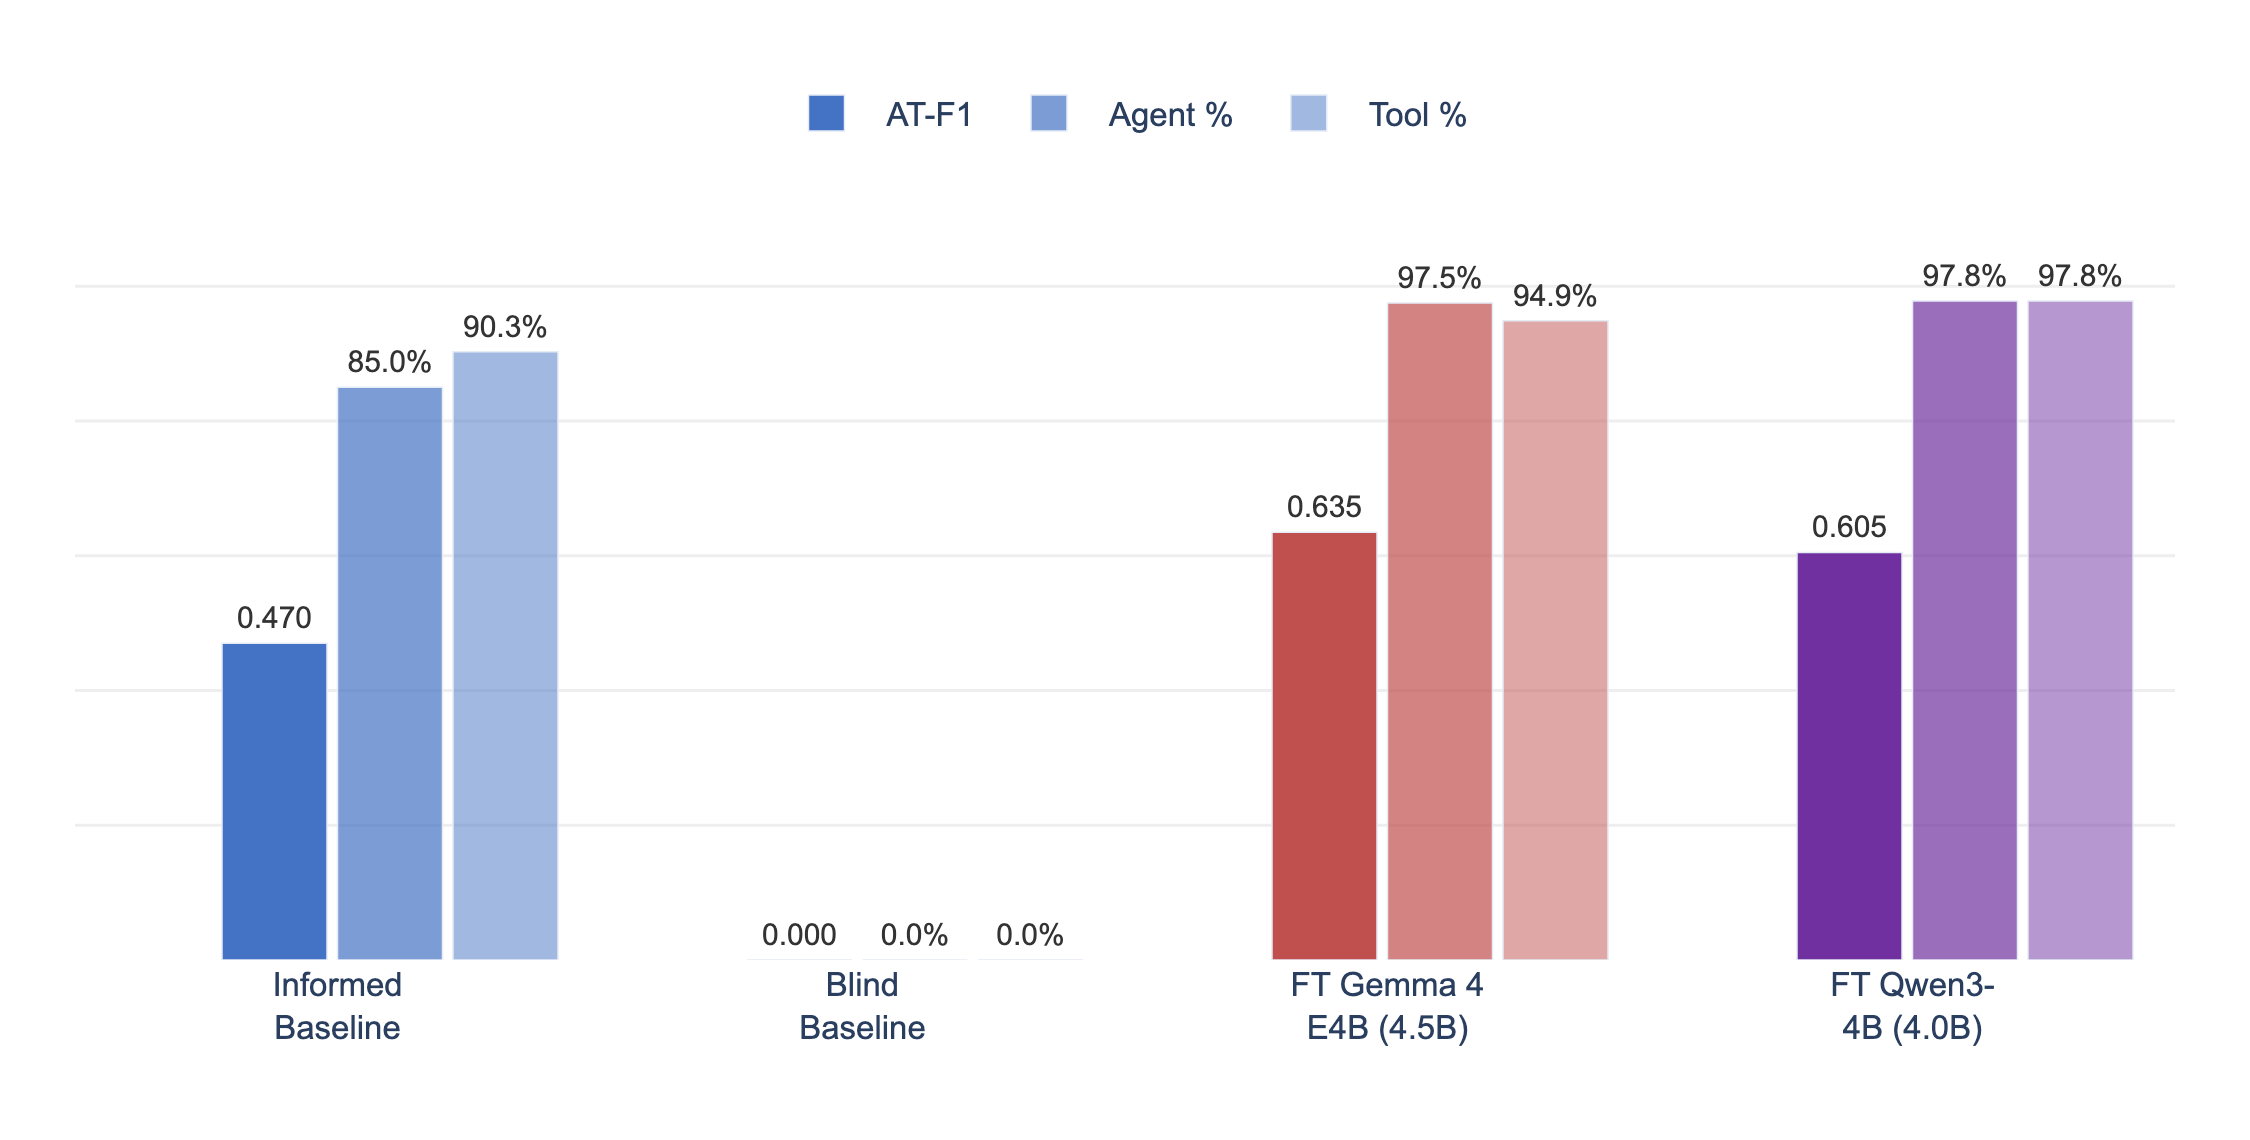
\includegraphics[width=\columnwidth]{figures/main_results_bar.png}
\caption{Structural planning metrics across all four configurations. Fine-tuned models operating without tool descriptions surpass the informed baseline on AT-F1, agent routing, and tool selection.}
\label{fig:main-results}
\end{figure}

\begin{figure}[t]
\centering
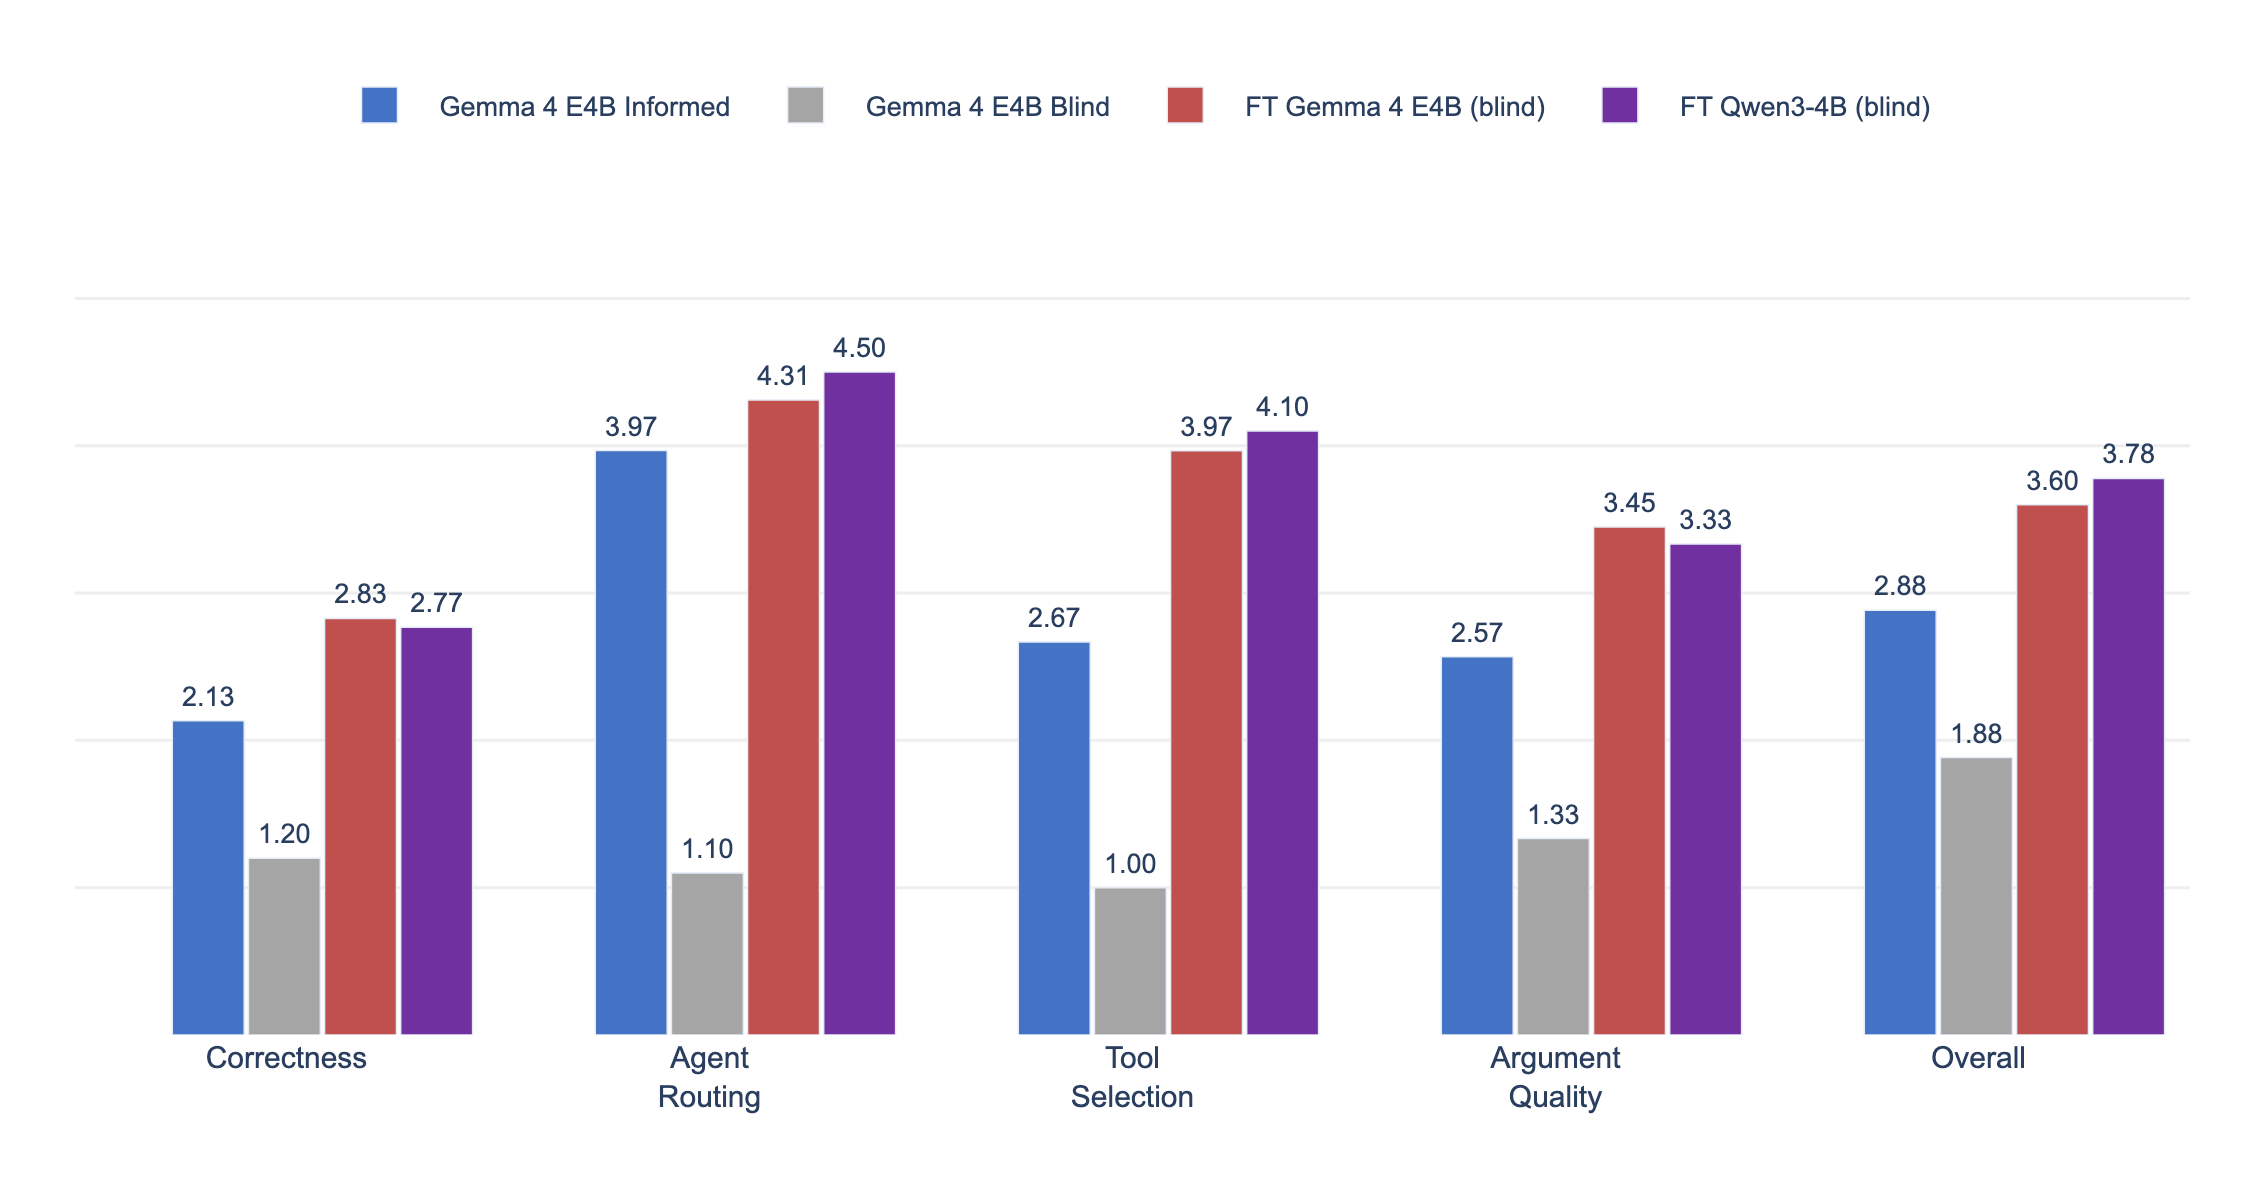
\includegraphics[width=\columnwidth]{figures/judge_scores_bar.png}
\caption{LLM-as-judge scores (1--5 scale) across five evaluation dimensions. Fine-tuned models operating without tool descriptions outperform the informed baseline on every dimension, with the largest gains on tool selection and agent routing.}
\label{fig:judge-scores}
\end{figure}

The fine-tuned Gemma model reaches AT-F1 of 0.635 compared with 0.470 for the informed baseline, with agent routing at 97.5\% and tool selection at 94.9\%. The fine-tuned Qwen3 model achieves AT-F1 of 0.605 and the highest judge overall score of 3.78 (vs.\ 2.88 informed, 1.88 description-free). Both fine-tuned models reach 95--98\% on agent and tool accuracy.

\textbf{Metric agreement.} The structural metrics and the LLM-judge scores show strong directional agreement across all four configurations. Each metric family has known limitations: AT-F1 is deterministic but penalizes valid alternative plans; LLM-judge scores capture semantic quality but may exhibit grading bias. The fact that both independently rank the configurations in the same order---description-free baseline worst, informed baseline second, fine-tuned Gemma third, fine-tuned Qwen3 best on judge score---provides stronger evidence than either metric alone.

Because the 1--5 judge scale has a floor of 1.0, the description-free baseline's score of 1.88 corresponds to 0.88/4.0 on a zero-anchored scale, confirming near-complete failure.

\begin{figure}[t]
\centering
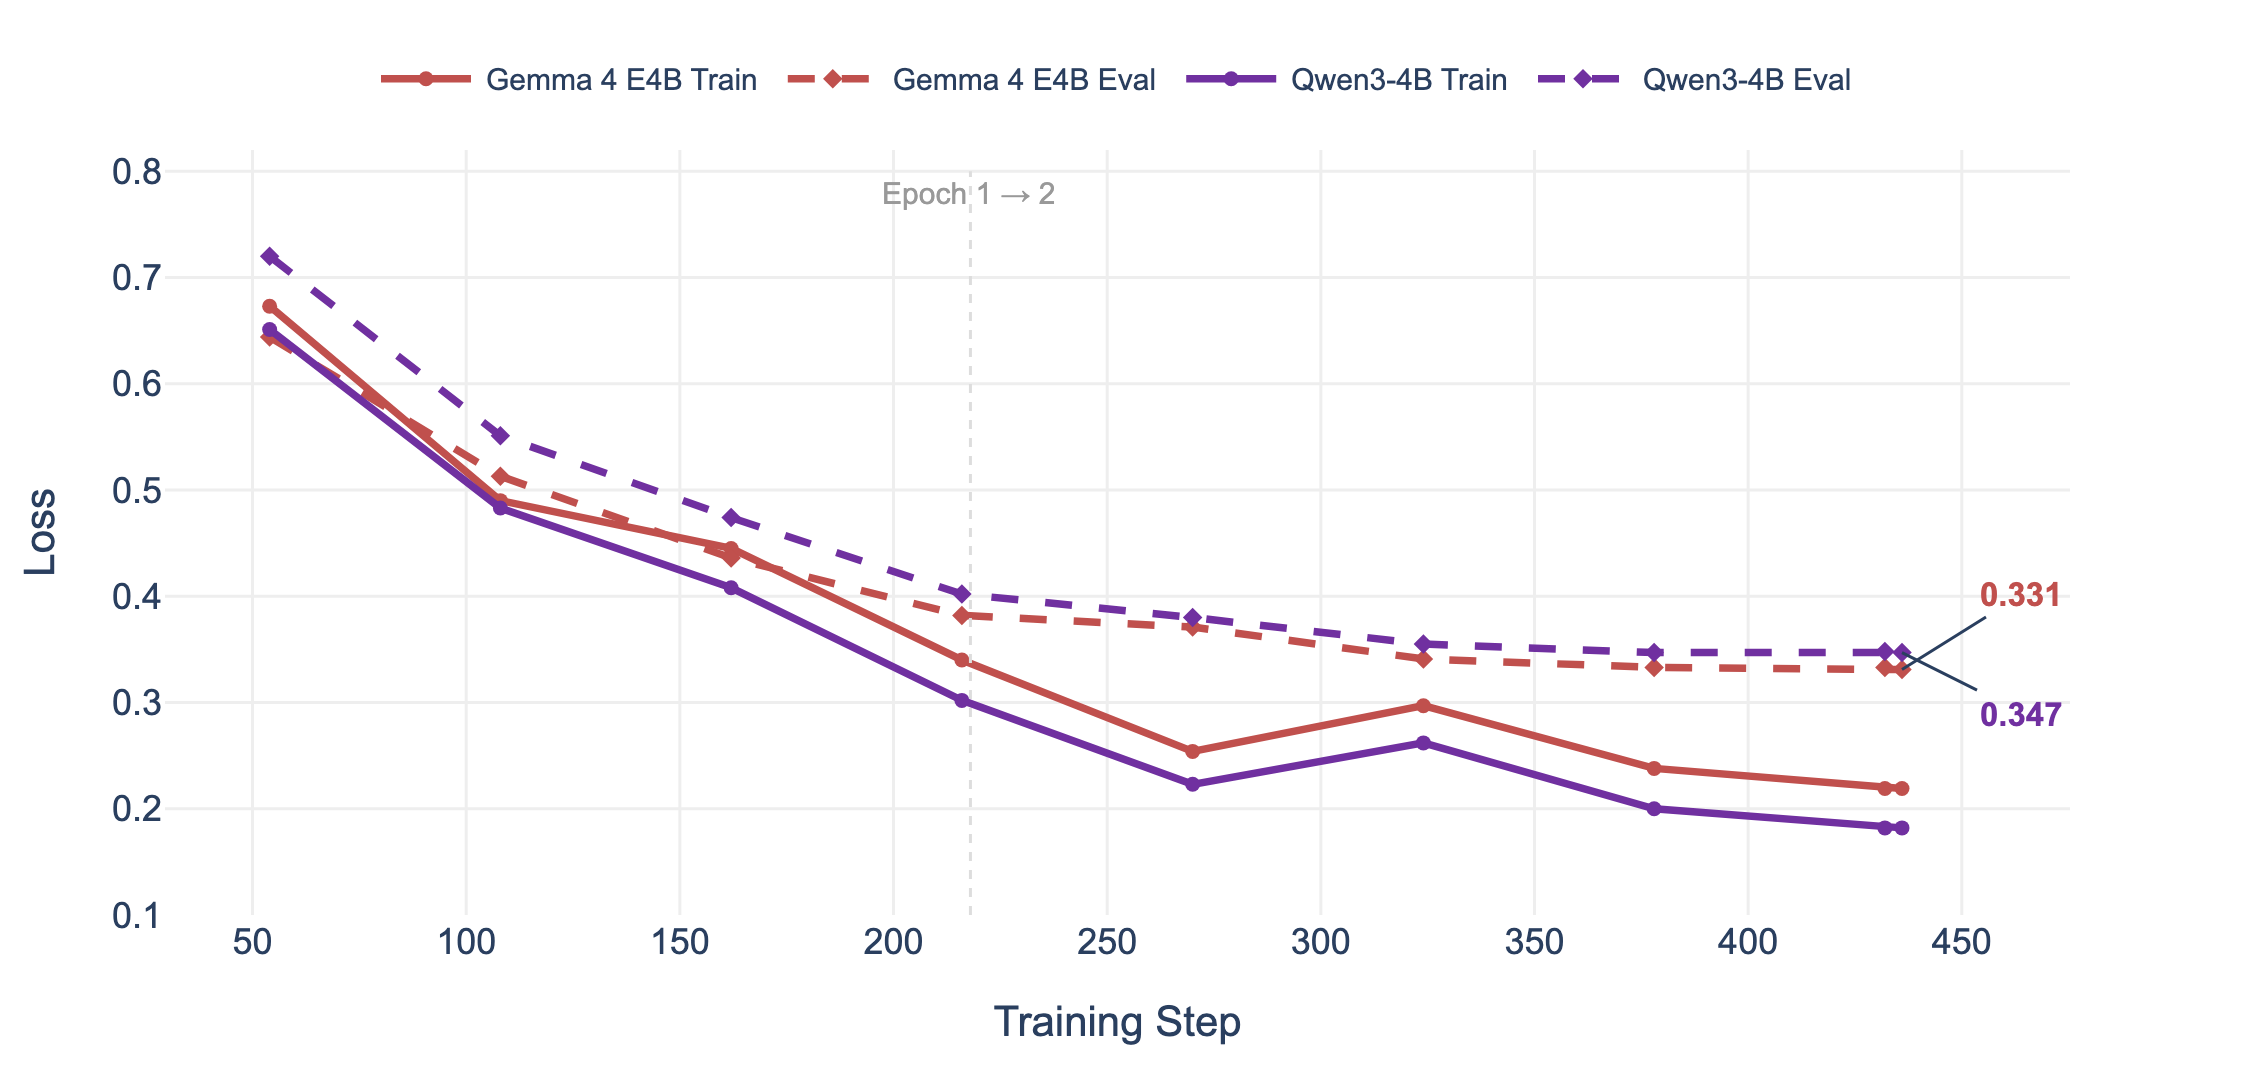
\includegraphics[width=\columnwidth]{figures/training_curves.png}
\caption{Training and evaluation loss over 436 steps (2 epochs). Both models converge smoothly to comparable final evaluation losses (Gemma 0.331, Qwen3 0.347), despite Qwen3 starting from a higher initial loss.}
\label{fig:training-curves}
\end{figure}

Fig.~\ref{fig:training-curves} shows that both models converge smoothly within two epochs, with no sign of training instability. Despite starting from a higher initial loss, Qwen3 converges to a comparable final evaluation loss (0.347 vs.\ 0.331 for Gemma), indicating that both architectures are well suited for this task. Qwen3's higher judge score (3.78 vs.\ 3.60) despite similar eval loss suggests that its native tool-calling tokens may provide structural advantages that are not fully captured by cross-entropy loss alone.

The practical token savings are substantial: description-free inference after fine-tuning reduces input length from $\sim$2,400 tokens to $\sim$128 tokens---an 82.6\% reduction measured from end-to-end execution. A preliminary 10-scenario pilot further validated that plan quality correlates with execution success (70\% task completion).


\subsection{LoRA Rank Selection}
\label{sec:lora-rank}

Having established that fine-tuning enables description-free inference that surpasses the informed baseline, we next investigate how the adapter capacity affects planning quality. The LoRA rank $r$ controls the number of trainable parameters and thus the model's capacity to absorb new tool-use knowledge. We sweep $r \in \{8, 16, 32, 64\}$ on Gemma~4~E4B, corresponding to trainable-parameter fractions from 0.32\% to 2.51\%.

\begin{figure}[t]
\centering
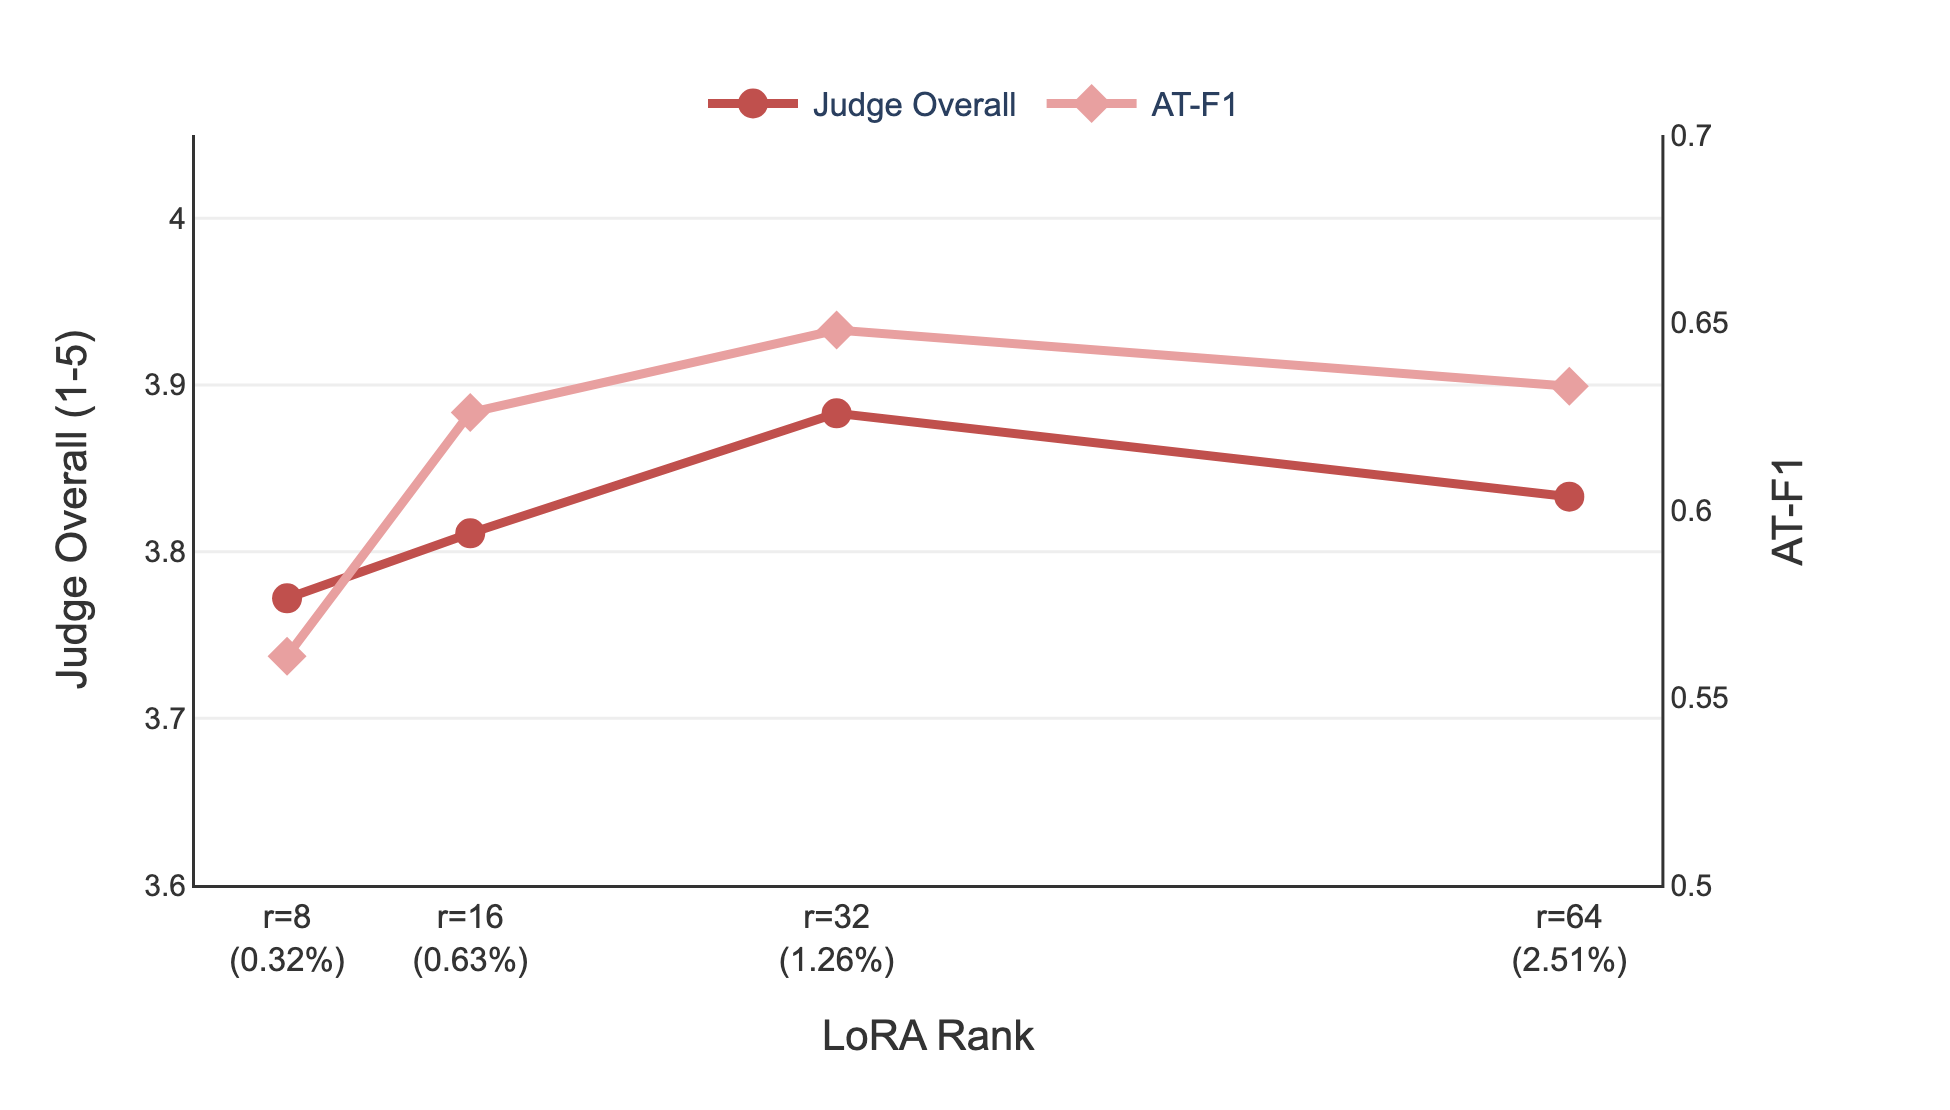
\includegraphics[width=\columnwidth]{figures/lora_rank_ablation.png}
\caption{Effect of LoRA rank on planning quality (Gemma~4~E4B). Both Judge Overall (left axis) and AT-F1 (right axis) peak at $r$=32 and decline at $r$=64, suggesting diminishing returns at higher adapter capacity.}
\label{fig:lora-rank}
\end{figure}

As shown in Fig.~\ref{fig:lora-rank}, both metrics rise steeply from $r$=8 (Judge 3.77, AT-F1 0.56) to $r$=16 (3.81, 0.63) and peak at $r$=32 (3.88, 0.65). At $r$=64 performance slightly degrades (3.83, 0.63), suggesting that 2.51\% trainable parameters exceeds the useful capacity for this task and may lead to overfitting. This finding is important for the forgetting analysis in Section~\ref{sec:forgetting}: while $r$=32 maximizes planning quality, smaller ranks preserve more general knowledge.


\subsection{Profiling}
\label{sec:profiling}

Beyond planning quality, deployment requires understanding computational cost. We profiled both models on a single A100 80GB GPU to compare memory footprint, training time, and inference throughput. Table~\ref{tab:profiling-comparison} summarizes the results.

\begin{table}[t]
\centering
\caption{Profiling comparison on A100 80GB}
\label{tab:profiling-comparison}
\begin{tabular}{lccc}
\hline
\textbf{Metric} & \textbf{Gemma} & \textbf{Qwen3} & \textbf{Ratio} \\
\hline
Base memory (8-bit) & 11.5\,GB & 4.42\,GB & 0.38$\times$ \\
Peak training memory & 24.1\,GB & 16.06\,GB & 0.67$\times$ \\
Training time (2 epochs) & 56\,min & 39.7\,min & 0.71$\times$ \\
Inference speed & 1.4\,tok/s & 3.49\,tok/s & 2.49$\times$ \\
Eval time (30 scenarios) & 59\,min & 40.7\,min & 0.69$\times$ \\
Best eval loss & 0.331 & 0.347 & 1.05$\times$ \\
\hline
\end{tabular}

\vspace{0.3em}
\begin{minipage}{0.95\columnwidth}
\footnotesize
Ratios show Qwen3 relative to Gemma (lower is better for memory/time; higher for speed).
\end{minipage}
\end{table}

Qwen3 uses 62\% less base memory, trains 29\% faster, and runs 2.5$\times$ faster at inference. Both models reach comparable final evaluation losses (Gemma 0.331, Qwen3 0.347). The main CUDA bottleneck was \texttt{MatMul8bitLt}, which accounted for 56.3\% of total CUDA time. Qwen3's speed advantage comes directly from having fewer total parameters (4.0B vs.\ 8.0B), which reduces the size of every 8-bit matrix multiplication. The total cost of all experiments was approximately \$62 in A100 GPU compute (Gemini API costs for training-data generation and LLM-judge evaluation are excluded). Appendix~D provides full profiling details including the CUDA operator breakdown and cost estimation.


\subsection{Catastrophic Forgetting}
\label{sec:forgetting}

A critical concern for production deployment is whether tool-use fine-tuning degrades the model's general reasoning capabilities. We evaluate this using a 100-question multiple-choice benchmark spanning three domains: MMLU (40 questions covering computer science, geography, logic, marketing, and general knowledge), ARC-Challenge (30 grade-school science reasoning questions), and HellaSwag (30 commonsense sentence-completion questions). These benchmarks are entirely independent of AssetOpsBench and test capabilities that should be unaffected by tool-planning fine-tuning. Connecting to the LoRA rank results from Section~\ref{sec:lora-rank}, we test both $r$=8 (the lean adapter) and $r$=32 (the quality-optimal adapter) on Gemma, and $r$=32 on Qwen3. Full benchmark composition, subject selection rationale, and evaluation protocol are in Appendix~\ref{app:forgetting}.

\begin{figure}[t]
\centering
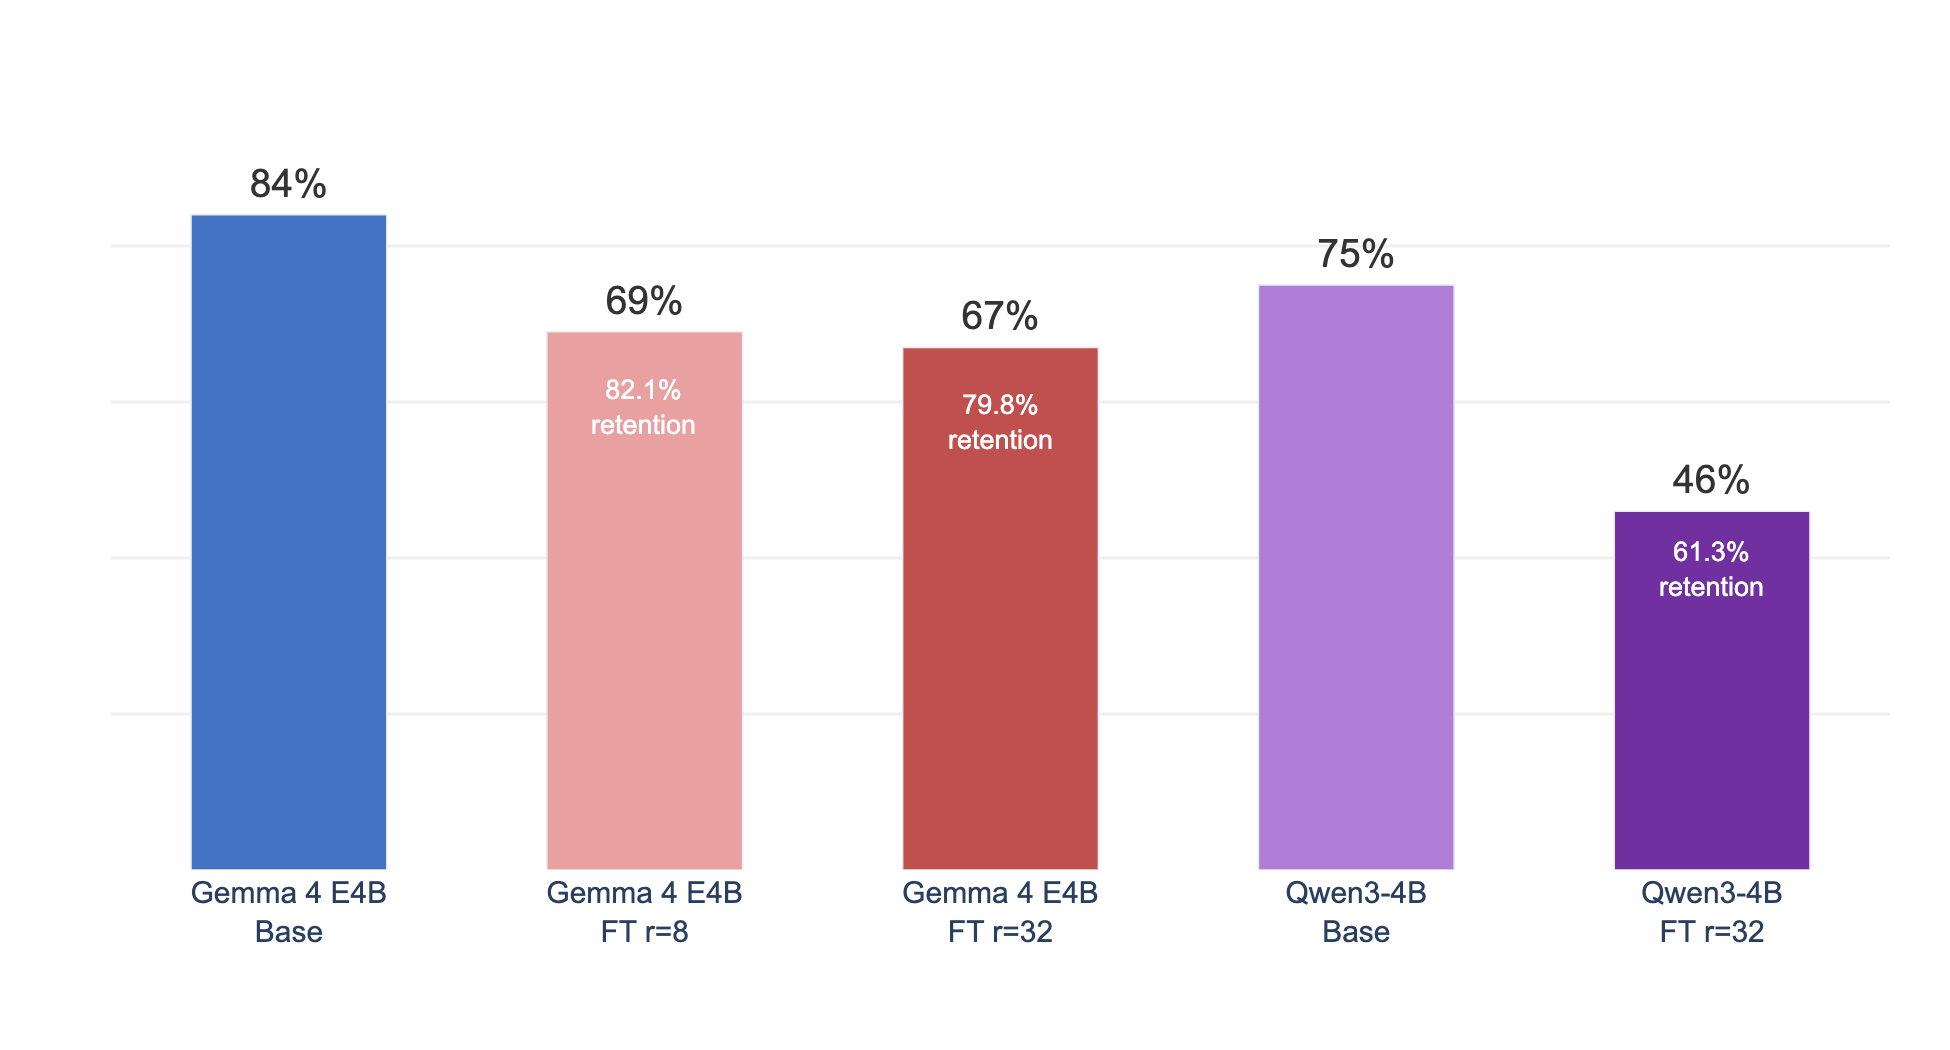
\includegraphics[width=\columnwidth]{figures/forgetting_overall.png}
\caption{Overall MCQ accuracy before and after tool-use fine-tuning. Gemma~4~E4B (blue/red) retains 79.8--82.1\% of base performance; Qwen3-4B (purple) retains only 61.3\%. Retention percentages shown inside bars. Per-benchmark breakdown in Appendix~\ref{app:forgetting}.}
\label{fig:forgetting}
\end{figure}

As shown in Fig.~\ref{fig:forgetting}, Gemma shows moderate forgetting: the base model scores 84.0\% MCQ accuracy, dropping to 69.0\% at $r$=8 (82.1\% retention) and 67.0\% at $r$=32 (79.8\% retention). Per-question analysis reveals that Gemma at $r$=32 forgot 21 of 100 questions while learning 4 new ones. This reveals a quality--retention trade-off: Section~\ref{sec:lora-rank} showed that $r$=32 achieves the best judge score (3.88 vs.\ 3.77 for $r$=8), but at the cost of 2.3 percentage points of retention. For deployment where general reasoning matters, the smaller $r$=8 adapter may be preferable.

Qwen3 exhibits substantially worse forgetting. Its base model scores 75.0\% MCQ accuracy, which drops to 46.0\% after fine-tuning---a retention of only 61.3\%. Per-question analysis shows Qwen3 forgot 36 questions while learning only 7 new ones. This reveals a fundamental trade-off: Qwen3 achieves the highest planning quality (judge 3.78) but the worst knowledge retention. A likely contributing factor is the trainable-parameter ratio: with the same LoRA rank $r$=32, Qwen3 updates 1.62\% of its parameters compared with only 0.63\% for Gemma. However, other differences---GQA vs.\ hybrid attention, different pretraining corpora, and a smaller vocabulary (152K vs.\ 262K)---also affect retention, so the parameter ratio cannot be isolated as the sole cause. We did not run Qwen3 at $r$=8 due to compute constraints; if the parameter ratio were the dominant factor, Qwen3 at $r$=8 ($\sim$0.41\% trainable) should show retention closer to Gemma at $r$=8 (0.32\%), but architectural differences may prevent full convergence. Matching LoRA rank does not imply matching adaptation intensity across architectures of different sizes.

The per-benchmark breakdown (Fig.~\ref{fig:forgetting-detail} in Appendix~\ref{app:forgetting}) reveals that Qwen3's forgetting is especially severe on logical reasoning (75\%$\rightarrow$25\%) and commonsense completion (50\%$\rightarrow$27\%), while Gemma's degradation is more evenly distributed across domains.

We verified that forgetting was not caused by inference quantization: the base Gemma model achieved 84\% in bf16 and 87\% in 8-bit (this small reversal is within noise for a 100-question benchmark), confirming that quantization alone does not explain the 84\%$\rightarrow$67\% degradation observed after fine-tuning.


\subsection{Additional Ablations}
\label{sec:ablation-highlights}

Training data composition had a substantial effect on planning quality. Plan-only data (Config~A) achieved the highest judge score of 3.90, outperforming Tool+Plan (Config~C) at 3.60. This is because every planning example implicitly demonstrates which agents and tools to use, encoding tool knowledge through usage rather than explicit description. Tool-only data (Config~B) scored only 2.59, confirming that tool definitions alone do not transfer to realistic planning. Our attempt to enrich the training set with explicit tool-knowledge examples did not improve planning quality, suggesting that for structured planning tasks, demonstration-based learning is more effective than declarative knowledge injection. See Appendix~B (Fig.~\ref{fig:data-ablation}).

Quantization had minimal effect: 8-bit and 4-bit produced judge scores of 3.78 and 3.74 respectively. See Appendix~C.


%===========================================================================
\section{Discussion}
%===========================================================================

\subsection{Interpretation}

The fine-tuned models operating without tool descriptions provide the strongest overall balance between tool-selection accuracy, argument quality, plan structure, and token efficiency. A single model trained across the full mixture of tool-use examples can learn shared planning patterns that transfer across IoT, FMSR, TSFM, WorkOrder, and multiagent scenarios, without requiring separate models for each domain. The consistent results across both structural and LLM-judge evaluation approaches suggest that the improvement is genuine and not an artifact of a single metric.

The fact that fine-tuned models outperform the informed baseline \emph{without any tool descriptions} suggests that tool schemas are not always best used as prompt-time context. We attribute this to two mechanisms. First, \emph{context competition}: tool descriptions consume 82.6\% of input tokens, leaving limited context for the actual query. Small models have limited attention capacity and may struggle to attend to relevant query details amid verbose schema text. Second, \emph{pretraining distribution mismatch}: the base model was pretrained on general text, not structured tool schemas. Parsing unfamiliar schema formats at inference time is a separate challenge from planning itself. Fine-tuning removes both burdens by internalizing tool knowledge into the model parameters, freeing the full context window for task-relevant information.

The Qwen3 results show that model architecture affects how well tool knowledge is internalized. Despite having fewer parameters, Qwen3 achieves a higher judge score (3.78 vs.\ 3.60) while reaching a comparable evaluation loss (0.347 vs.\ 0.331). One possible explanation is that Qwen3's native \texttt{<tool\_call>} tokens provide structural priors for tool-use generation. Another is that its standard GQA attention is more amenable to LoRA adaptation than Gemma's hybrid sliding-window and global attention design.

However, the forgetting results reveal that stronger planning quality can come at the cost of reduced general knowledge retention. Gemma retains 67--69\% MCQ accuracy after fine-tuning, while Qwen3 drops to 46.0\% despite its higher judge score. The trainable-parameter ratio (1.62\% vs.\ 0.63\%) is a likely contributing factor, though architectural differences between the two models also play a role (Section~\ref{sec:forgetting}). This is a cautionary finding---higher planning quality may come with greater forgetting, especially in smaller models. In production, this could be mitigated through lower LoRA ranks, adapter merging, selective LoRA freezing, or replay-based continual learning.


\subsection{Limitations}

All experiments were conducted on AssetOpsBench, so it remains unclear whether the same internalization behavior would generalize to other benchmarks or tool catalogs. The evaluation set is small (30 held-out scenarios), and performance differences may have wide confidence intervals. These findings should be interpreted as a proof of concept.

We did not evaluate fine-tuned models with tool descriptions included in the prompt, which would isolate whether the improvement comes from internalization itself or from freeing context-window capacity that was previously consumed by schema text. Our benchmark coverage is incomplete: five of seven or more AssetOpsBench agent families were used, with VibrationAgent excluded and WorkOrderAgent untested in full execution. Our evaluation focuses on plan quality rather than full end-to-end task completion, and we did not complete curriculum-learning or continual-learning experiments.


\subsection{Future Work}

Future work should evaluate the fine-tuned models inside a complete agent loop, measuring task success, latency, and robustness. Our 10-scenario pilot showed 70\% task completion correlating with plan quality, but a larger benchmark is needed.

A second direction is continual learning: testing whether a model can incrementally internalize new tools without forgetting old ones. A concrete experiment is a VibrationAgent hold-out study, training first without VibrationAgent examples and then incrementally adding them.

The benchmark scope should be expanded to include the additional 162+ scenarios and all 9 asset classes. Finally, since \texttt{MatMul8bitLt} dominates CUDA time, future work should investigate GPTQ- or AWQ-style kernels to improve inference speed.


%===========================================================================
\section{Conclusion}
%===========================================================================

We demonstrated that QLoRA fine-tuning enables $\sim$4B parameter models to internalize MCP tool descriptions, eliminating 82.6\% of prompt tokens while improving planning quality. On AssetOpsBench, fine-tuned Gemma~4~E4B achieves a judge score of 3.60 (vs.\ 2.88 for the informed baseline) and Qwen3-4B achieves 3.78 with 62\% less memory and $2.5\times$ faster inference. We find that LoRA rank $r$=32 optimizes planning quality, while smaller ranks ($r$=8) offer better general-knowledge retention with only modest quality reduction, suggesting a tunable quality--retention trade-off. The cost of fine-tuning is moderate forgetting---79.8\% MCQ retention for Gemma, 61.3\% for Qwen3---governed by the trainable-parameter ratio. The total experiment cost of \$62 on A100 demonstrates the accessibility of this approach.


\section*{AI Disclosure}

Our team used AI tools, including ChatGPT, Gemini, and Claude, to help write and run specific tests and to polish the writing in this paper. All research decisions, ideas, analysis, and conclusions are our own.


%===========================================================================
\appendix
%===========================================================================

\section{Training Data Composition}
\label{app:data}

\begin{table}[!htbp]
\centering
\caption{Three training datasets}
\label{tab:three-training-datasets}
\footnotesize
\setlength{\tabcolsep}{3pt}
\renewcommand{\arraystretch}{1.15}
\begin{tabular}{p{0.23\columnwidth}p{0.13\columnwidth}p{0.27\columnwidth}p{0.27\columnwidth}}
\hline
\textbf{Dataset} & \textbf{N} & \textbf{Source} & \textbf{Description} \\
\hline
Tool Knowledge
& $\sim$500
& Gemini 2.5 Flash
& Tool taxonomy, ownership, args, routing, hard negatives \\
Planning
& $\sim$1,200
& Gold plans + paraphrases
& Scenario $\rightarrow$ concise planning steps \\
Execution
& $\sim$100
& Gold plans + traces
& Scenario $\rightarrow$ planning + execution links \\
\hline
\end{tabular}

\vspace{0.3em}
\begin{minipage}{0.95\columnwidth}
\footnotesize
\textit{Note.} Total $\sim$1,833 examples. Config~C (Tool+Plan) uses $\sim$1,741 after 95/5 train/eval split.
\end{minipage}
\end{table}


\section{Training Data Ablation}
\label{app:data-ablation}

We compare four data configurations using 8-bit QLoRA with $r$=32 on Gemma~4~E4B. Fig.~\ref{fig:data-ablation} shows the results.

\begin{figure}[!htbp]
\centering
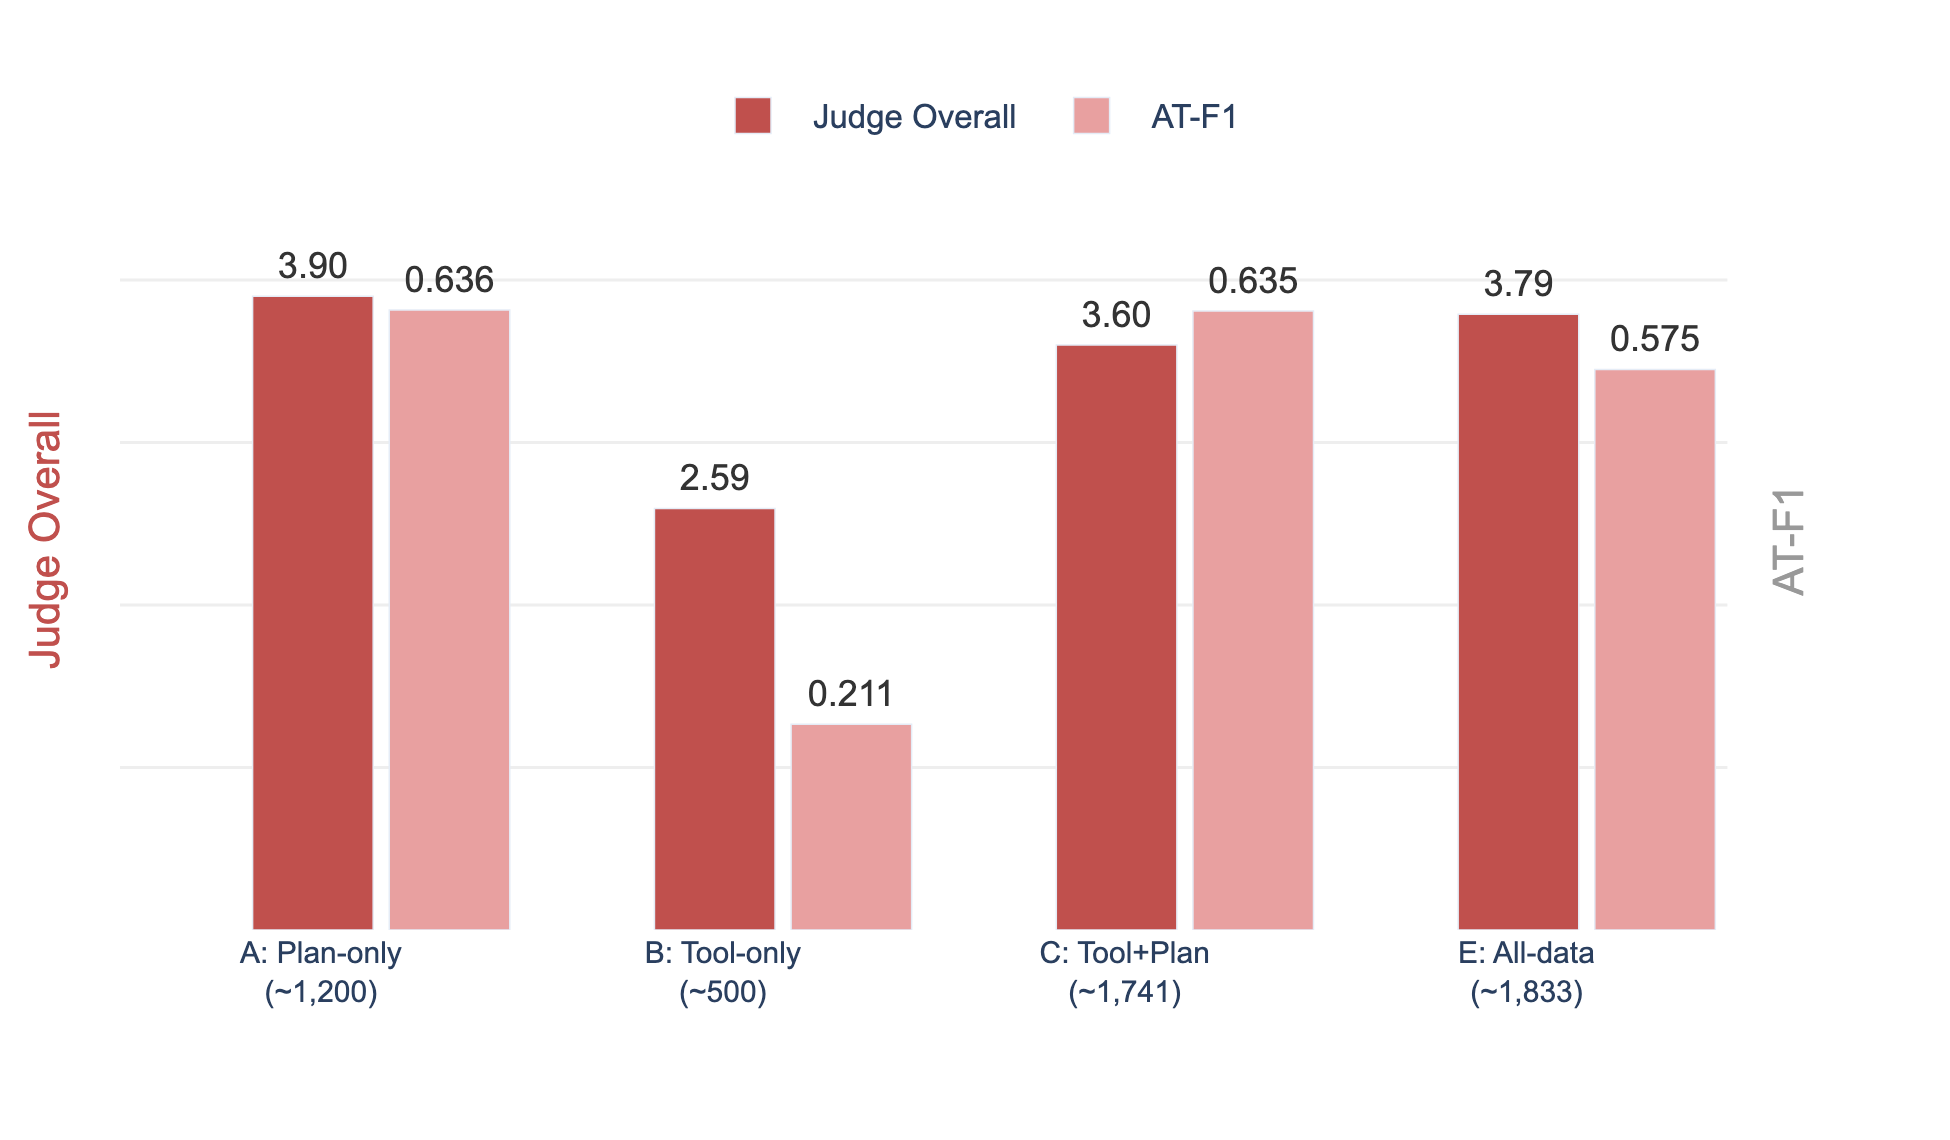
\includegraphics[width=\columnwidth]{figures/data_ablation.png}
\caption{Effect of training data composition on planning quality. Plan-only data achieves the highest judge score (3.90), while Tool-only data performs poorly (2.59).}
\label{fig:data-ablation}
\end{figure}

Plan-only training (Config~A, $\sim$1,200 examples) achieves the highest judge score of 3.90 and AT-F1 of 0.636. Adding tool-knowledge examples (Config~C) does not improve judge quality (3.60), and tool-only training (Config~B) performs poorly (2.59). Despite Config~A's higher judge score, we use Config~C as the primary configuration because it provides broader tool-knowledge coverage and the highest tool selection accuracy (94.9\% vs.\ 92.9\%).

\FloatBarrier


\section{Quantization Ablation}
\label{app:quant}

\begin{table}[!htbp]
\centering
\caption{Quantization ablation (Gemma 4 E4B, $r$=32)}
\label{tab:quantization-ablation}
\footnotesize
\begin{tabular}{lccc}
\hline
\textbf{Quantization} & \textbf{AT-F1} & \textbf{Judge} & \textbf{Train Time} \\
\hline
8-bit (bitsandbytes) & 0.617 & 3.78 & 56\,min \\
4-bit NF4 (double quant.) & 0.642 & 3.74 & $\sim$50\,min \\
\hline
\end{tabular}

\vspace{0.3em}
\begin{minipage}{0.95\columnwidth}
\footnotesize
\textit{Note.} Differences are marginal. We use 8-bit as the default for its higher judge score.
\end{minipage}
\end{table}

\FloatBarrier


\section{Profiling Details}
\label{app:profiling}

All profiling was conducted on a single NVIDIA A100 80GB GPU. Fig.~\ref{fig:profiling} provides a visual comparison; Tables~\ref{tab:cuda-breakdown} and~\ref{tab:cost-breakdown} provide additional detail.

\begin{figure}[!htbp]
\centering
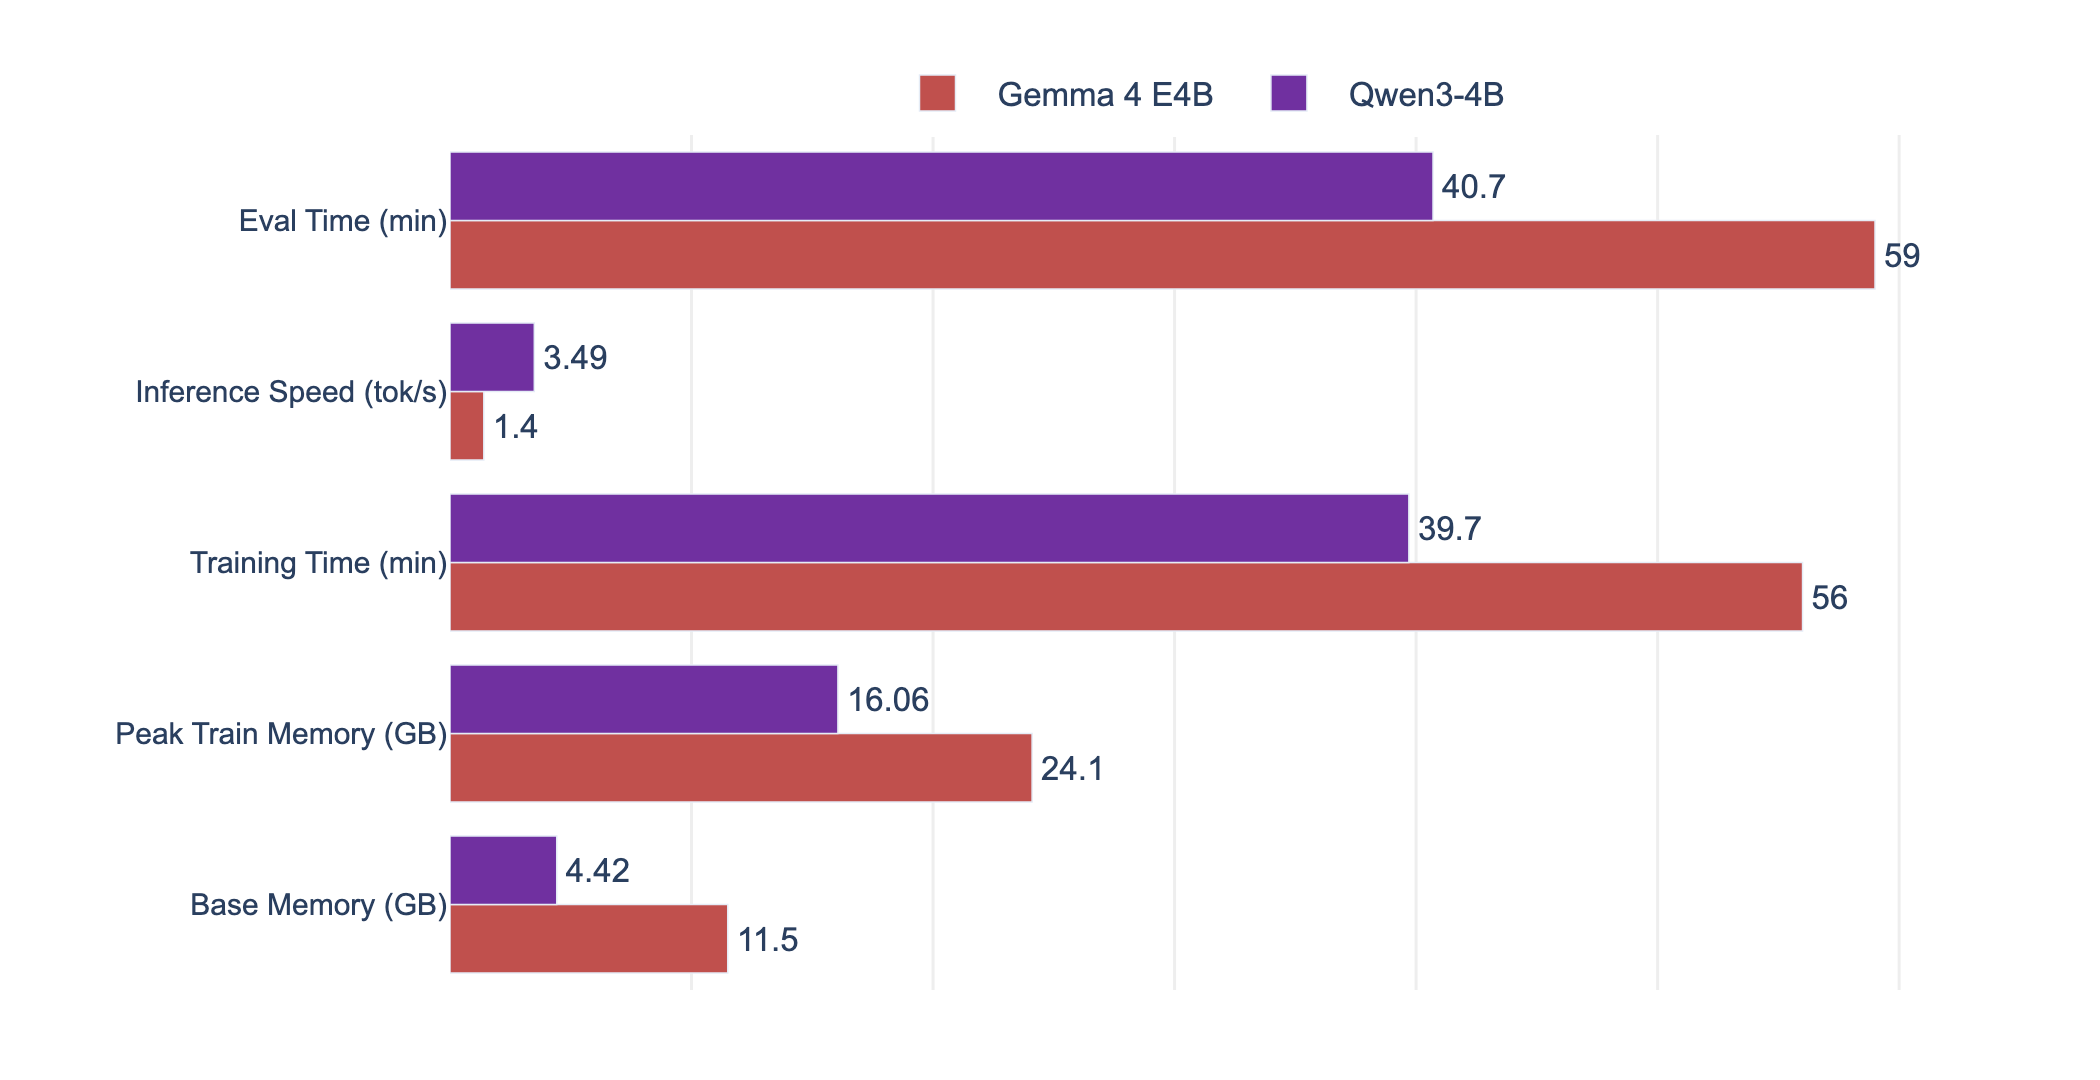
\includegraphics[width=\columnwidth]{figures/profiling_comparison.png}
\caption{Profiling comparison between Gemma~4~E4B and Qwen3-4B. Qwen3 uses less memory, trains faster, and achieves 2.5$\times$ higher inference throughput.}
\label{fig:profiling}
\end{figure}

Training throughput scaled from $\sim$886 tok/s at batch size 1 to $\sim$1,415 tok/s at batch size 4, beyond which the model exceeded available memory.

\begin{table}[!htbp]
\centering
\caption{CUDA operator breakdown (Gemma inference, 64 tokens)}
\label{tab:cuda-breakdown}
\footnotesize
\begin{tabular}{lc}
\hline
\textbf{Operation} & \textbf{\% CUDA Time} \\
\hline
\texttt{MatMul8bitLt} & 56.3\% \\
\texttt{aten::mm} & 18.2\% \\
\texttt{scaled\_dot\_product\_attention} & 8.7\% \\
Other (softmax, layer\_norm, etc.) & 16.8\% \\
\hline
\end{tabular}

\vspace{0.3em}
\begin{minipage}{0.95\columnwidth}
\footnotesize
\textit{Note.} The 8-bit matmul kernel dominates inference time. Qwen3 achieves 2.5$\times$ higher throughput because its smaller parameter count reduces the size of every matmul.
\end{minipage}
\end{table}

\begin{table}[!htbp]
\centering
\caption{Experiment cost breakdown (A100 at \$3.93/hr)}
\label{tab:cost-breakdown}
\footnotesize
\begin{tabular}{lcc}
\hline
\textbf{Component} & \textbf{A100 Hours} & \textbf{Cost} \\
\hline
Gemma ablations (rank, data, quant) & 3.1 & \$12.18 \\
Qwen3 training + eval & 1.5 & \$5.78 \\
Forgetting analysis (MCQ + judge) & 11.2 & \$44.00 \\
\hline
\textbf{Total} & \textbf{$\sim$15.8} & \textbf{$\sim$\$62} \\
\hline
\end{tabular}
\end{table}

\FloatBarrier


\section{Judge Prompts}
\label{app:judge}

\subsection{Plan Quality Judge}

We use Gemini 2.5 Flash (temperature=0, max\_tokens=8192) to evaluate each candidate plan against the gold reference. The prompt provides the question, gold plan, candidate plan, and tool inventory, and asks the judge to rate on a 1--5 scale across six dimensions: correctness, agent routing, tool selection, argument quality, efficiency, and dependency correctness. Each dimension includes a rubric (5 = matches gold reference, 3 = partially correct, 1 = major errors). The judge returns a JSON object with integer scores.

\subsection{MCQ Forgetting Judge}

For the forgetting benchmark, we use Gemini 2.5 Flash (temperature=0, max\_tokens=1024). The prompt provides the question, answer choices, correct answer, and the model's full response. The judge is instructed to look at the \emph{final} answer the model commits to, ignoring intermediate reasoning, and return a JSON object with a binary correct/incorrect grade. This approach is more reliable than token-level evaluation because instruction-tuned models produce chain-of-thought reasoning before committing to an answer letter.

\FloatBarrier


\section{Forgetting Benchmark Details}
\label{app:forgetting}

\begin{table}[!htbp]
\centering
\caption{Retention benchmark composition}
\label{tab:retention-benchmark-composition}
\footnotesize
\begin{tabular}{lcl}
\hline
\textbf{Source} & \textbf{N} & \textbf{Description} \\
\hline
MMLU (5 subjects) & 40 & Knowledge and reasoning \\
ARC-Challenge & 30 & Grade-school science \\
HellaSwag & 30 & Commonsense completion \\
\hline
Total & 100 & \\
\hline
\end{tabular}
\end{table}

\begin{figure}[!htbp]
\centering
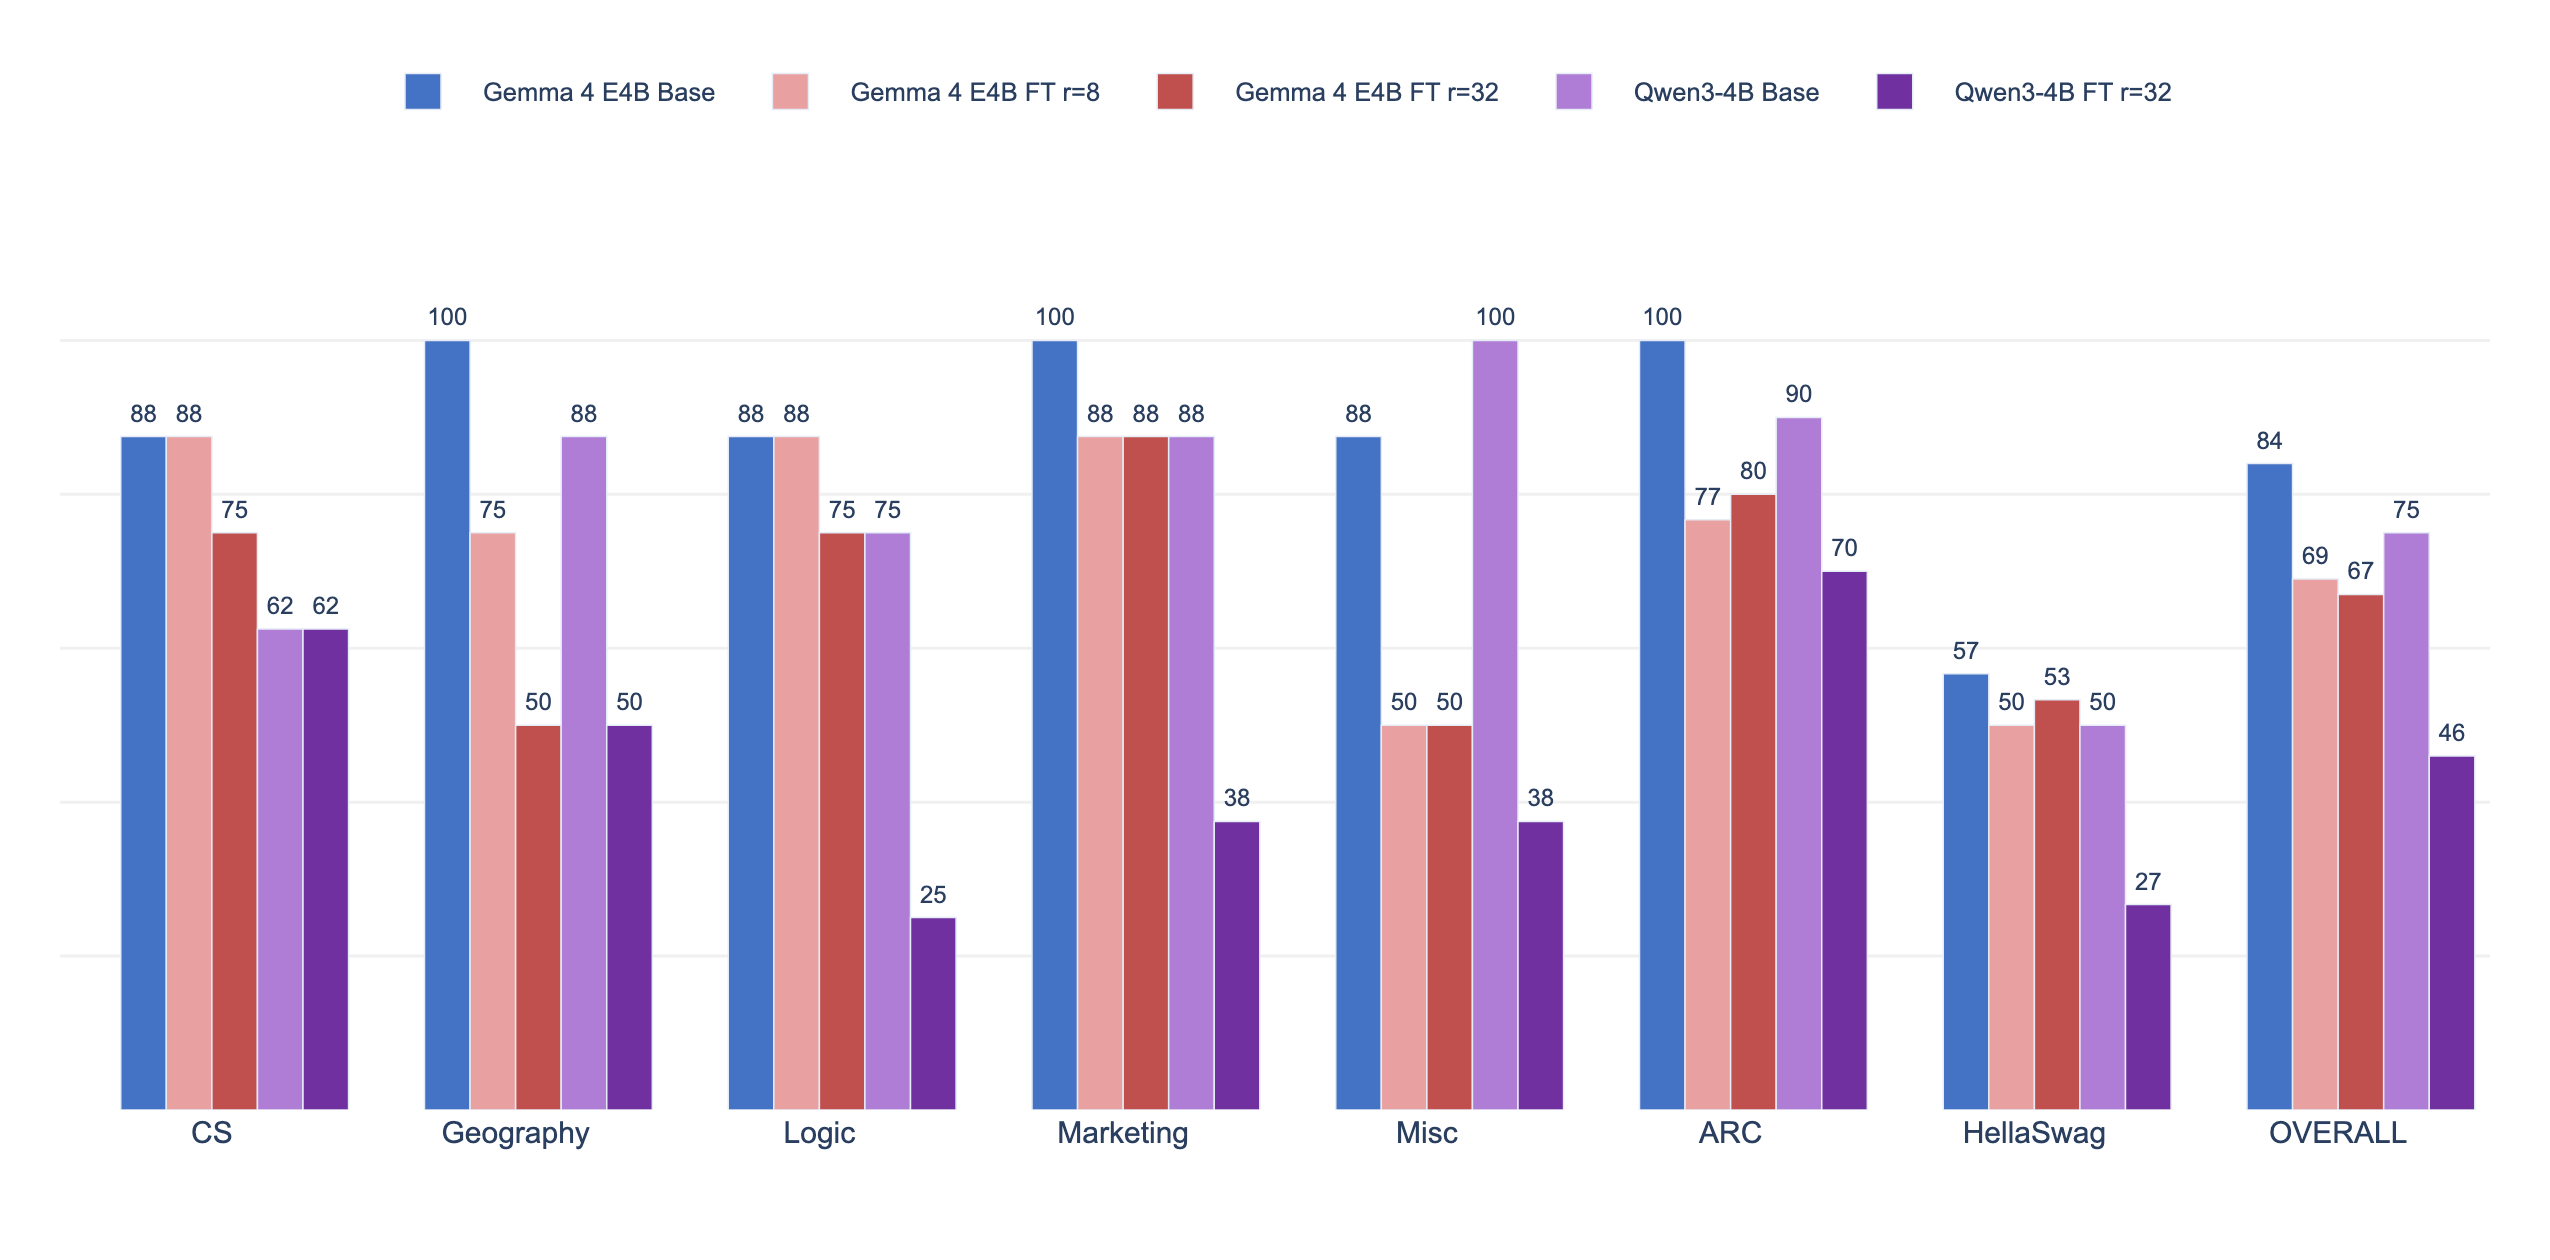
\includegraphics[width=\columnwidth]{figures/forgetting_per_benchmark.png}
\caption{Per-benchmark MCQ accuracy for base and fine-tuned models. Qwen3-4B (purple) shows severe degradation on Logic (75\%$\rightarrow$25\%), Marketing (88\%$\rightarrow$38\%), and HellaSwag (50\%$\rightarrow$27\%). Gemma forgetting is more uniform across benchmarks.}
\label{fig:forgetting-detail}
\end{figure}

MMLU subjects are selected for a suitable difficulty range on $\sim$4B models (base accuracy 40--100\%): High School Computer Science, High School Geography, Logical Fallacies, Marketing, and Miscellaneous. We avoid niche subjects where the base model scores near zero, making retention difficult to interpret.

The evaluation protocol is fixed across all models: 100 MCQ examples loaded with a fixed random seed; the model is prompted to think step by step and provide a final answer letter (A/B/C/D); generation is capped at 512 tokens; Gemini judges correctness. Overall retention = FT accuracy / base accuracy.

\clearpage

\section{Example Prompt and Gold Plan}
\label{app:prompt-example}

We show a concrete example of the informed planning prompt and corresponding gold plan for AssetOpsBench scenario~114.

\textbf{Question:} ``What are the failure modes of Chiller 6 that can be identified by analyzing the data from the available sensors?''

\vspace{0.5em}
\textbf{Informed prompt} (as sent to the model, $\sim$2,400 tokens total):

\begin{lstlisting}
You are a planning assistant for industrial
asset operations and maintenance.

Decompose the question below into a sequence
of subtasks. For each subtask, assign an agent
and select the exact tool to call with its
arguments.

Available agents and tools:

IoTAgent:
  - sites(): Retrieves a list of sites. Each
    site is represented by a name.
  - assets(site_name: string): Returns a list
    of assets for a given site. Each asset
    includes an id and a name.
  - sensors(site_name: string, asset_id:
    string): Lists the sensors available for
    a specified asset at a given site.
  - history(site_name: string, asset_id:
    string, start: string, final: string):
    Returns historical sensor values for
    the specified asset(s) within a time range.

FMSRAgent:
  - get_failure_modes(asset_name: string):
    Returns a list of known failure modes
    for the given asset.
  - get_failure_mode_sensor_mapping(asset_name:
    string, failure_modes: list, sensors:
    list): For each (failure_mode, sensor)
    pair determines whether the sensor can
    detect the failure. Returns a bidirectional
    mapping plus per-pair relevancy details.

TSFMAgent:
  - get_ai_tasks(): Returns the list of
    supported AI task types.
  - get_tsfm_models(): Returns available
    pre-trained TTM model checkpoints.
  - run_tsfm_forecasting(model_id: string,
    data: string, ...): Run zero-shot
    time-series forecasting.
  - run_tsfm_finetuning(model_id: string,
    data: string, ...): Fine-tune TSFM models.
  - run_tsad(data: string, ...): Run
    time-series anomaly detection.
  - run_integrated_tsad(data: string, ...):
    Run integrated anomaly detection with
    forecasting context.

Utilities:
  - json_reader(file_name: string): Reads a
    JSON file and returns the parsed data.
  - current_date_time(): Provides the current
    date and time as a JSON object.
  - current_time_english(): Returns the
    current time in English text.

[Output format specification and rules omitted
 for brevity -- see Section III-A]

Question: What are the failure modes of
Chiller 6 that can be identified by analyzing
the data from the available sensors?

Plan:
\end{lstlisting}

\vspace{0.5em}
\textbf{Gold plan} (4 steps, produced by Gemini 2.5 Flash):

\begin{lstlisting}
#Task1: Retrieve the list of assets for the
  "MAIN" site to find "Chiller 6" and its
  corresponding asset ID.
#Agent1: IoTAgent
#Tool1: assets
#Args1: {"site_name": "MAIN"}
#Dependency1: None
#ExpectedOutput1: A list of assets, including
  their IDs and names, from which the asset
  ID for "Chiller 6" will be extracted.

#Task2: Get the list of all available sensors
  for "Chiller 6" using its asset ID and
  site name.
#Agent2: IoTAgent
#Tool2: sensors
#Args2: {"site_name": "MAIN",
  "asset_id": "{step_1}"}
#Dependency2: #S1
#ExpectedOutput2: A list of sensor objects
  associated with "Chiller 6".

#Task3: Identify the known failure modes for
  "Chiller 6".
#Agent3: FMSRAgent
#Tool3: get_failure_modes
#Args3: {"asset_name": "Chiller 6"}
#Dependency3: None
#ExpectedOutput3: A list of known failure mode
  strings for "Chiller 6".

#Task4: Determine which of the identified
  failure modes can be detected by the
  available sensors of "Chiller 6".
#Agent4: FMSRAgent
#Tool4: get_failure_mode_sensor_mapping
#Args4: {"asset_name": "Chiller 6",
  "failure_modes": "{step_3}",
  "sensors": "{step_2}"}
#Dependency4: #S2, #S3
#ExpectedOutput4: A bidirectional mapping
  showing which failure modes can be detected
  by which sensors, along with relevancy
  details.
\end{lstlisting}

In the description-free setting, the entire tool catalog (IoTAgent through Utilities, $\sim$2,200 tokens) is removed from the prompt. The fine-tuned model must produce the same structured plan from only the question text and output format specification.

\FloatBarrier


\begin{thebibliography}{00}

\bibitem{b1} Model Context Protocol, ``What is the Model Context Protocol (MCP)?'' Model Context Protocol Documentation. [Online]. Available: https://modelcontextprotocol.io/docs/getting-started/intro. Accessed: Apr. 30, 2026.

\bibitem{b2} D. C. Patel, S. Lin, J. T. Rayfield, N. Zhou, R. Vaculin, N. Martinez, F. O'Donncha, and J. Kalagnanam, ``AssetOpsBench: Benchmarking AI Agents for Task Automation in Industrial Asset Operations and Maintenance,'' submitted to ICLR 2026, OpenReview, Sept. 2025. [Online]. Available: https://openreview.net/forum?id=ld6JUQbhes.

\bibitem{b3} T. Dettmers, A. Pagnoni, A. Holtzman, and L. Zettlemoyer, ``QLoRA: Efficient Finetuning of Quantized LLMs,'' in \textit{Advances in Neural Information Processing Systems}, vol. 36, 2023.

\bibitem{b4} E. J. Hu, Y. Shen, P. Wallis, Z. Allen-Zhu, Y. Li, S. Wang, L. Wang, and W. Chen, ``LoRA: Low-Rank Adaptation of Large Language Models,'' in \textit{International Conference on Learning Representations}, 2022.

\bibitem{b5} Google DeepMind, ``Gemini 2.5 Flash and 2.5 Flash Image Model Card,'' 2025. [Online]. Available: https://storage.googleapis.com/deepmind-media/Model-Cards/Gemini-2-5-Flash-Model-Card.pdf. Accessed: Apr. 30, 2026.

\bibitem{b6} Google AI for Developers, ``Gemma 4 model overview,'' Google AI for Developers Documentation, 2026. [Online]. Available: https://ai.google.dev/gemma/docs/core. Accessed: Apr. 30, 2026.

\bibitem{b7} J. Han, L. Du, H. Du, X. Zhou, Y. Wu, W. Zheng, and D. Han, ``SLIM: Let LLM Learn More and Forget Less with Soft LoRA and Identity Mixture,'' in \textit{Proceedings of the 2025 Conference of the Nations of the Americas Chapter of the Association for Computational Linguistics: Human Language Technologies}, 2025.

\bibitem{b8} T. Schick, J. Dwivedi-Yu, R. Dess\`i, R. Raileanu, M. Lomeli, E. Hambro, L. Zettlemoyer, N. Cancedda, and T. Scialom, ``Toolformer: Language Models Can Teach Themselves to Use Tools,'' \textit{arXiv preprint arXiv:2302.04761}, 2023.

\bibitem{b9} S. G. Patil, T. Zhang, X. Wang, and J. E. Gonzalez, ``Gorilla: Large Language Model Connected with Massive APIs,'' \textit{arXiv preprint arXiv:2305.15334}, 2023.

\bibitem{b10} Y. Qin, S. Liang, Y. Ye, K. Zhu, L. Yan, Y. Lu, Y. Lin, X. Cong, X. Tang, B. Qian, S. Zhao, L. Hong, R. Tian, R. Xie, J. Zhou, M. Gerstein, D. Li, Z. Liu, and M. Sun, ``ToolLLM: Facilitating Large Language Models to Master 16000+ Real-world APIs,'' \textit{arXiv preprint arXiv:2307.16789}, 2023.

\bibitem{b11} H. Jiang, Q. Wu, C.-Y. Lin, Y. Yang, and L. Qiu, ``LLMLingua: Compressing Prompts for Accelerated Inference of Large Language Models,'' in \textit{Proceedings of the 2023 Conference on Empirical Methods in Natural Language Processing}, 2023.

\bibitem{b12} C.-Y. Hsieh, C.-L. Li, C.-K. Yeh, H. Nakhost, Y. Fujii, A. Ratner, R. Krishna, C.-Y. Lee, and T. Pfister, ``Distilling Step-by-Step! Outperforming Larger Language Models with Less Training Data and Smaller Model Sizes,'' \textit{arXiv preprint arXiv:2305.02301}, 2023.

\bibitem{b13} L. Zheng, W.-L. Chiang, Y. Sheng, S. Zhuang, Z. Wu, Y. Zhuang, Z. Lin, Z. Li, D. Li, E. P. Xing, H. Zhang, J. E. Gonzalez, and I. Stoica, ``Judging LLM-as-a-Judge with MT-Bench and Chatbot Arena,'' \textit{arXiv preprint arXiv:2306.05685}, 2023.

\bibitem{b14} D. Hendrycks, C. Burns, S. Basart, A. Zou, M. Mazeika, D. Song, and J. Steinhardt, ``Measuring Massive Multitask Language Understanding,'' \textit{arXiv preprint arXiv:2009.03300}, 2020.

\bibitem{b15} P. Clark, I. Cowhey, O. Etzioni, T. Khot, A. Sabharwal, C. Schoenick, and O. Tafjord, ``Think you have Solved Question Answering? Try ARC, the AI2 Reasoning Challenge,'' \textit{arXiv preprint arXiv:1803.05457}, 2018.

\bibitem{b16} R. Zellers, A. Holtzman, Y. Bisk, A. Farhadi, and Y. Choi, ``HellaSwag: Can a Machine Really Finish Your Sentence?,'' in \textit{Proceedings of the 57th Annual Meeting of the Association for Computational Linguistics}, 2019.

\bibitem{b17} Qwen Team, ``Qwen3 Technical Report,'' Alibaba Group, 2025. [Online]. Available: https://qwenlm.github.io/blog/qwen3/. Accessed: May 6, 2026.

\end{thebibliography}

\end{document}
